%File: formatting-instructions-latex-2024.tex
%release 2024.0
\documentclass[letterpaper]{article} % DO NOT CHANGE THIS
\usepackage{aaai24}  % DO NOT CHANGE THIS
\usepackage{times}  % DO NOT CHANGE THIS
\usepackage{helvet}  % DO NOT CHANGE THIS
\usepackage{courier}  % DO NOT CHANGE THIS
\usepackage[hyphens]{url}  % DO NOT CHANGE THIS
\usepackage{graphicx} % DO NOT CHANGE THIS
\urlstyle{rm} % DO NOT CHANGE THIS
\def\UrlFont{\rm}  % DO NOT CHANGE THIS
\usepackage{natbib}  % DO NOT CHANGE THIS AND DO NOT ADD ANY OPTIONS TO IT
\usepackage{caption} % DO NOT CHANGE THIS AND DO NOT ADD ANY OPTIONS TO IT
\frenchspacing  % DO NOT CHANGE THIS
\setlength{\pdfpagewidth}{8.5in}  % DO NOT CHANGE THIS
\setlength{\pdfpageheight}{11in}  % DO NOT CHANGE THIS
%
% These are recommended to typeset algorithms but not required. See the subsubsection on algorithms. Remove them if you don't have algorithms in your paper.
\usepackage{algorithm}
\usepackage{algorithmic}

% additional packages
\usepackage{makecell}
\usepackage{booktabs}
\usepackage[table,xcdraw]{xcolor}
\usepackage{multirow}
\usepackage{amssymb}
\usepackage{amsmath}

\def\eg{e.g.} \def\Eg{E.g.}
\def\ie{i.e.} \def\Ie{I.e.}
\def\cf{c.f.} \def\Cf{C.f.}

%
% These are are recommended to typeset listings but not required. See the subsubsection on listing. Remove this block if you don't have listings in your paper.
\usepackage{newfloat}
\usepackage{listings}
\DeclareCaptionStyle{ruled}{labelfont=normalfont,labelsep=colon,strut=off} % DO NOT CHANGE THIS
\lstset{%
	basicstyle={\footnotesize\ttfamily},% footnotesize acceptable for monospace
	numbers=left,numberstyle=\footnotesize,xleftmargin=2em,% show line numbers, remove this entire line if you don't want the numbers.
	aboveskip=0pt,belowskip=0pt,%
	showstringspaces=false,tabsize=2,breaklines=true}
\floatstyle{ruled}
\newfloat{listing}{tb}{lst}{}
\floatname{listing}{Listing}
%
% Keep the \pdfinfo as shown here. There's no need
% for you to add the /Title and /Author tags.

% DISALLOWED PACKAGES
% \usepackage{authblk} -- This package is specifically forbidden
% \usepackage{balance} -- This package is specifically forbidden
% \usepackage{color (if used in text)
% \usepackage{CJK} -- This package is specifically forbidden
% \usepackage{float} -- This package is specifically forbidden
% \usepackage{flushend} -- This package is specifically forbidden
% \usepackage{fontenc} -- This package is specifically forbidden
% \usepackage{fullpage} -- This package is specifically forbidden
% \usepackage{geometry} -- This package is specifically forbidden
% \usepackage{grffile} -- This package is specifically forbidden
% \usepackage{hyperref} -- This package is specifically forbidden
% \usepackage{navigator} -- This package is specifically forbidden
% (or any other package that embeds links such as navigator or hyperref)
% \indentfirst} -- This package is specifically forbidden
% \layout} -- This package is specifically forbidden
% \multicol} -- This package is specifically forbidden
% \nameref} -- This package is specifically forbidden
% \usepackage{savetrees} -- This package is specifically forbidden
% \usepackage{setspace} -- This package is specifically forbidden
% \usepackage{stfloats} -- This package is specifically forbidden
% \usepackage{tabu} -- This package is specifically forbidden
% \usepackage{titlesec} -- This package is specifically forbidden
% \usepackage{tocbibind} -- This package is specifically forbidden
% \usepackage{ulem} -- This package is specifically forbidden
% \usepackage{wrapfig} -- This package is specifically forbidden
% DISALLOWED COMMANDS
% \nocopyright -- Your paper will not be published if you use this command
% \addtolength -- This command may not be used
% \balance -- This command may not be used
% \baselinestretch -- Your paper will not be published if you use this command
% \clearpage -- No page breaks of any kind may be used for the final version of your paper
% \columnsep -- This command may not be used
% % \newpage -- No page breaks of any kind may be used for the final version of your paper
% \pagebreak -- No page breaks of any kind may be used for the final version of your paperr
% \pagestyle -- This command may not be used
% \tiny -- This is not an acceptable font size.
% \vspace{- -- No negative value may be used in proximity of a caption, figure, table, section, subsection, subsubsection, or reference
% \vskip{- -- No negative value may be used to alter spacing above or below a caption, figure, table, section, subsection, subsubsection, or reference

\setcounter{secnumdepth}{0} %May be changed to 1 or 2 if section numbers are desired.

% The file aaai24.sty is the style file for AAAI Press
% proceedings, working notes, and technical reports.
%

% Title

% Your title must be in mixed case, not sentence case.
% That means all verbs (including short verbs like be, is, using,and go),
% nouns, adverbs, adjectives should be capitalized, including both words in hyphenated terms, while
% articles, conjunctions, and prepositions are lower case unless they
% directly follow a colon or long dash
\title{Weakly Supervised Semantic Segmentation for Driving Scenes}
\author{
    %Authors
    % All authors must be in the same font size and format.
    Dongseob Kim\equalcontrib\textsuperscript{\rm 1},
    Seungho Lee\equalcontrib\textsuperscript{\rm 1},
    Junsuk Choe\textsuperscript{\rm 2},
    Hyunjung Shim\thanks{Hyunjung Shim is a corresponding author.}\textsuperscript{\rm 3}
}
\affiliations{
    %Afiliations
    \textsuperscript{\rm 1} Yonsei University, South Korea\\
    \textsuperscript{\rm 2} Sogang University, South Korea\\
    \textsuperscript{\rm 3} Korea Advanced Institute of Science \& Technology, South Korea\\
    \{kou.k, seungholee\}@yonsei.ac.kr, jschoe@sogang.ac.kr, kateshim@kaist.ac.kr
}

\begin{document}

\maketitle

\begin{abstract}
State-of-the-art techniques in weakly-supervised semantic segmentation (WSSS) using image-level labels exhibit severe performance degradation on driving scene datasets such as Cityscapes. To address this challenge, we develop a new WSSS framework tailored to driving scene datasets. Based on extensive analysis of dataset characteristics, we employ Contrastive Language-Image Pre-training (CLIP) as our baseline to obtain pseudo-masks. However, CLIP introduces two key challenges: (1) pseudo-masks from CLIP lack in representing small object classes, and (2) these masks contain notable noise. We propose solutions for each issue as follows. (1) We devise Global-Local View Training that seamlessly incorporates small-scale patches during model training, thereby enhancing the model's capability to handle small-sized yet critical objects in driving scenes (\eg, \textit{traffic light}). (2) We introduce Consistency-Aware Region Balancing (CARB), a novel technique that discerns reliable and noisy regions through evaluating the consistency between CLIP masks and segmentation predictions. It prioritizes reliable pixels over noisy pixels via adaptive loss weighting. Notably, the proposed method achieves 51.8\% mIoU on the Cityscapes test dataset, showcasing its potential as a strong WSSS baseline on driving scene datasets. Experimental results on CamVid and WildDash2 demonstrate the effectiveness of our method across diverse datasets, even with small-scale datasets or visually challenging conditions. The code is available at https://github.com/k0u-id/CARB.
\end{abstract}

\section{Introduction}

Recent advancements in weakly supervised semantic segmentation (WSSS) using image-level labels have demonstrated impressive results, achieving performance levels of over 90\% compared to full supervised models on the PASCAL VOC dataset~\cite{lee2022threshold,yoon2022adversarial}. Given this success, it is crucial to transfer the WSSS framework to driving scenes, which are a significant scenario in semantic segmentation. Obtaining pixel-level labels in driving scenes is prohibitively expensive, making label-efficient training methods imperative in this context. For instance, Cityscapes required 1.5 hours per image~\cite{cordts2016cityscapes}, while PASCAL VOC required 239.7 seconds per image~\cite{bearman2016s}.

However, when applied to driving scene datasets like Cityscapes, WSSS models exhibit significant performance degradation. \citeauthor{akiva2023single} attributed this issue to the specific characteristics of the dataset, such as small object size, a high number of objects in each image, and limited diversity in object appearance~\cite{akiva2023single}. However, they only reported this tendency implicitly. In our study, we explicitly compare the driving scene datasets to the existing benchmark datasets (\ie, PASCAL VOC and MS COCO). As a result, we find that the driving scenes datasets lack negative samples and exhibit a remarkably high level of co-occurrence among classes. This poses a challenge in identifying individual objects through image classification, which hinders the effectiveness of common WSSS baselines, such as class activation mapping (CAM).

Recently, Contrastive Language Image Pre-training (CLIP), a model trained on a massive set of 400 million image-text pairs, has remarkably performed in open vocabulary classification. Using the open vocabulary classification ability of CLIP, we can avoid the characteristic of the dataset degrading the classifier's performance. As a result, as opposed to CAM, the seed mask generated by CLIP better distinguishes the object regions on the driving dataset like Cityscapes. Despite the potential, it often fails to identify small objects and produces noisy masks (Fig.~\ref{fig:mask_resizencrop}~(a)).

In this paper, we present a novel WSSS framework for driving scene datasets, to address the above two challenges inherent in CLIP. Considering CLIP as a baseline mask generator, we propose (1) global-local view training to handle small-sized objects and (2) \textit{Consistency-Aware Region Balancing (CARB)} to mitigate the negative effects of noisy pseudo-masks. Firstly, we found a unique property of CLIP: it offers considerably different pseudo-masks across input scales. Based on this observation, we use both a local view (\ie, a small-sized patch) and a global view (\ie, an original-sized image) during model training for accurately detecting small but critical objects in driving scenes (\eg, \textit{traffic light}).

\begin{figure*}[t]
\begin{center}
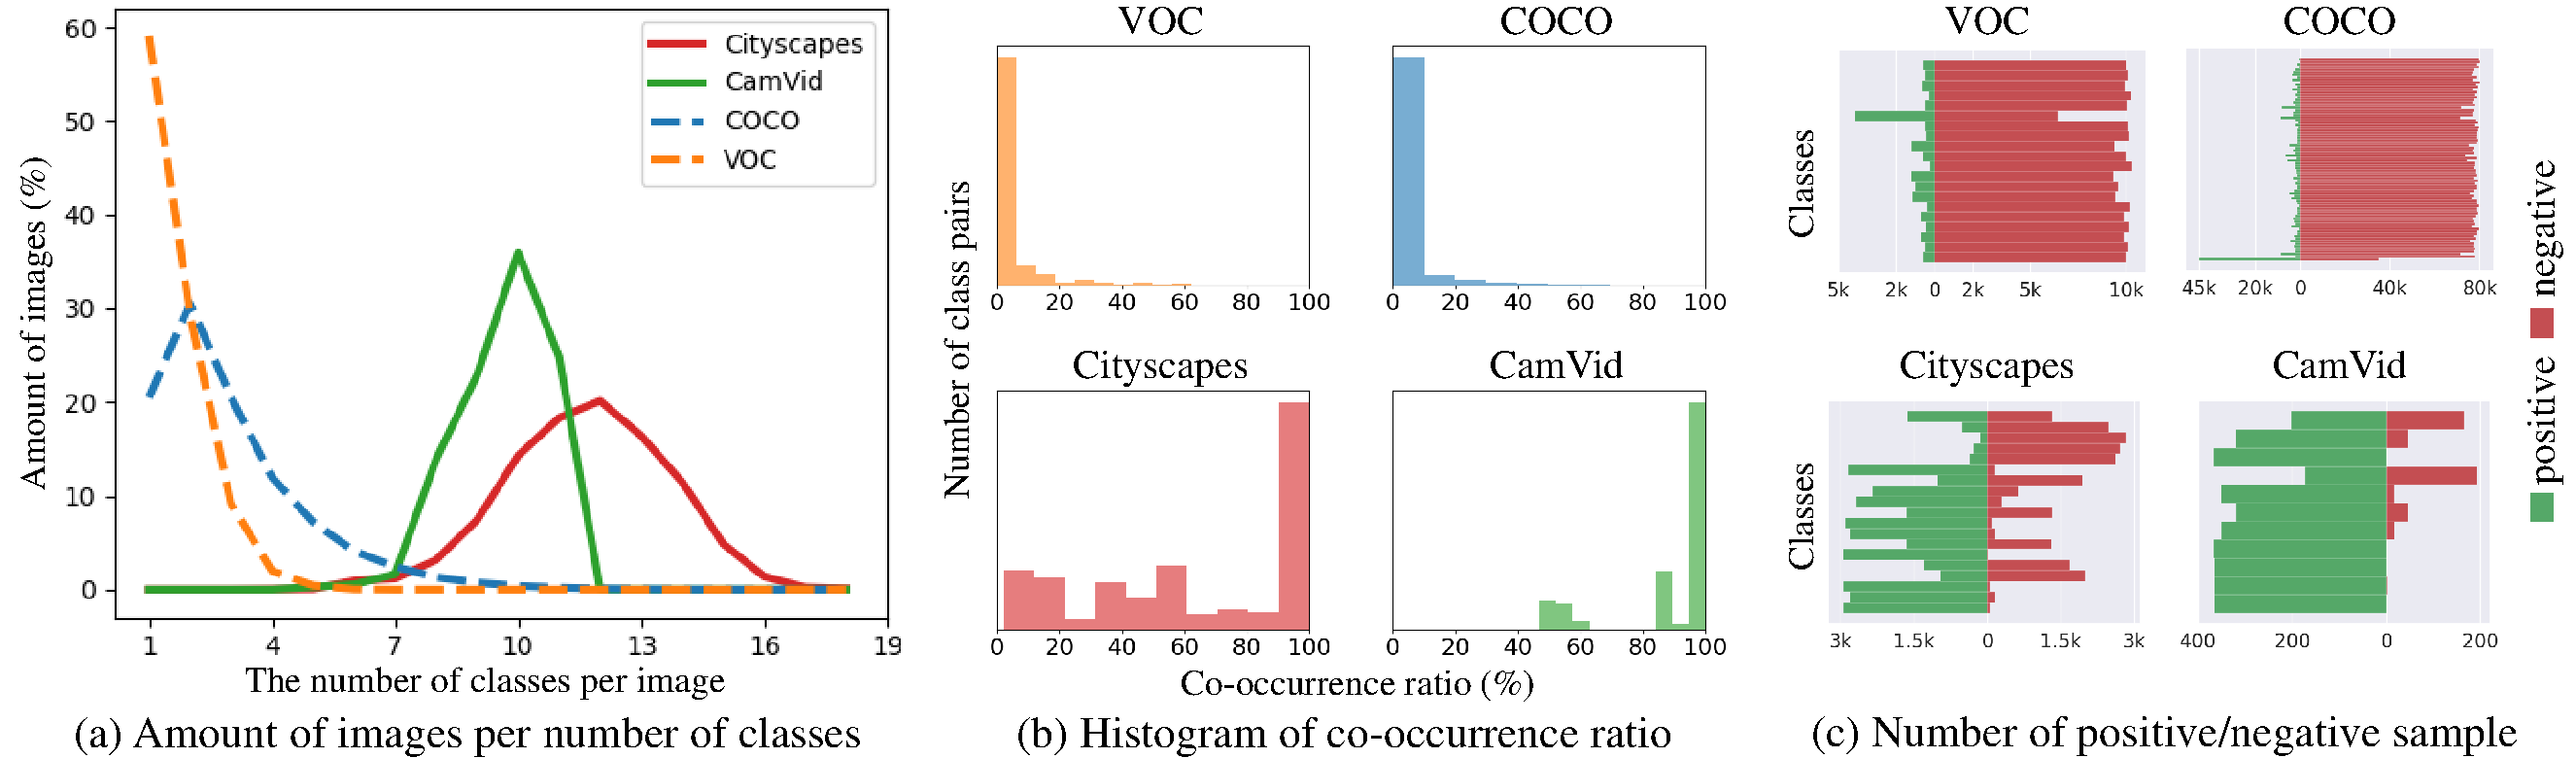
\includegraphics[width=17cm]{figures/fig_dataset.pdf}
\end{center}
\caption{Dataset statistics for Cityscapes, CamVid, MS COCO, and PASCAL VOC. (a) Counting the number of images given by the number of classes in a single image. (b) Histogram of co-occurrence ratio between classes. (c) The number of positive and negative images for each class.}
\label{fig:dataset}
\end{figure*}

Next, we propose CARB, which suppresses the erroneous region of pseudo-masks to train the segmentation model. Specifically, we divide the noisy pseudo-mask into consistent and inconsistent regions according to prediction consistency between the segmentation model and CLIP. The inconsistent region contains more false predictions than the consistent region, resulting in a higher loss. This discrepancy in the magnitude of loss values leads to a negative impact on the overall training process. To mitigate this, we propose a strategy to balance the losses from both regions, thereby suppressing the high loss of the inconsistent region.

In summary, we examine the distinct characteristics of driving scenes over the commonly evaluated datasets and highlight the issue of ineffective CAM-based approaches in these scenes. We introduce a new WSSS framework utilizing pseudo-masks generated from CLIP, suggesting global-local view training to handle small-sized objects and CARB to mitigate the negative effects of noisy pseudo-masks.

We demonstrate that the proposed method achieved 51.8\% mIoU on the Cityscapes dataset, showcasing the potential as a strong WSSS baseline for driving scenes. The effectiveness of the proposed method was confirmed on CamVid representing a small-scale dataset, and on WildDash2 containing more visually challenging scenes (\eg, diverse weather and lighting conditions). Owing to its advantage in performance and simple training, our method can serve as a valuable baseline for future research to address the challenges of WSSS in the driving scenes.

\section{Related Work}
\subsubsection{Earlier Works in WSSS.} Most WSSS techniques using image-level labels utilize CAM~\cite{zhou2016learning}. Due to its sparse coverage, recent studies have focused on expanding discriminative regions~\cite{jiang2019integral, wei2018revisiting, choe2019attention}. In terms of using global-local view, L2G~\cite{jiang2022l2g} strengthened classifier learning by using local attention. This method was also used to widen the discriminative region. Recently, some approaches have attempted to solve co-occurrence problem by incorporating additional information~\cite{lee2021railroad, lee2022weakly, Xie_2022_CVPR}. However, most of existing methods were only evaluated on PASCAL VOC~\cite{everingham2015pascal} or MS COCO~\cite{lin2014microsoft}. \citeauthor{akiva2023single}.~\citeyear{akiva2023single} conducted evaluations on more complex datasets like Cityscapes~\cite{cordts2016cityscapes} and ADE20k~\cite{zhou2019semantic}, but only revealed the performance limitations of existing WSSS studies. \citeauthor{wang2020deep}.~\citeyear{wang2020deep} introduced a clustering-based approach in driving scene datasets, while they only achieved a marginal improvement. Unlike most WSSS studies, we analyze distinct characteristics of the driving scene datasets compared to existing benchmark datasets and suggest a new direction for WSSS in driving scene scenarios.

\subsubsection{CLIP-based Segmentation.} CLIP~\cite{radford2021learning} is a framework trained on a large amount of image-text pairs. Several attempts have been made to utilize the characteristics of the multimodal embedding space in the field of segmentation~\cite{ding2022decoupling,Wang_2022_CVPR}. In WSSS, CLIMS~\cite{Xie_2022_CVPR} employed the embedding spaces by optimizing the mask based on the similarity between masked image and text embedding. CLIP-ES~\cite{Lin_2023_CVPR} generates seed masks in Grad-CAM manner~\cite{selvaraju2017grad}. Then, it refines masks with class-wise attention-based affinity of the CLIP image encoder.

Existing studies~\cite{li2022languagedriven, xu2021} have also shown a significant improvement in zero-shot and few-shot segmentation by leveraging CLIP's zero-shot ability. Recently, MaskCLIP~\cite{zhou2022extract} has been proposed to create dense masks from CLIP with category information at the dataset level rather than the image level. We employ MaskCLIP to extract dense labels from images and further propose a training strategy for handling the noise present in its pseudo-masks.

\begin{figure*}[t!]
\centering
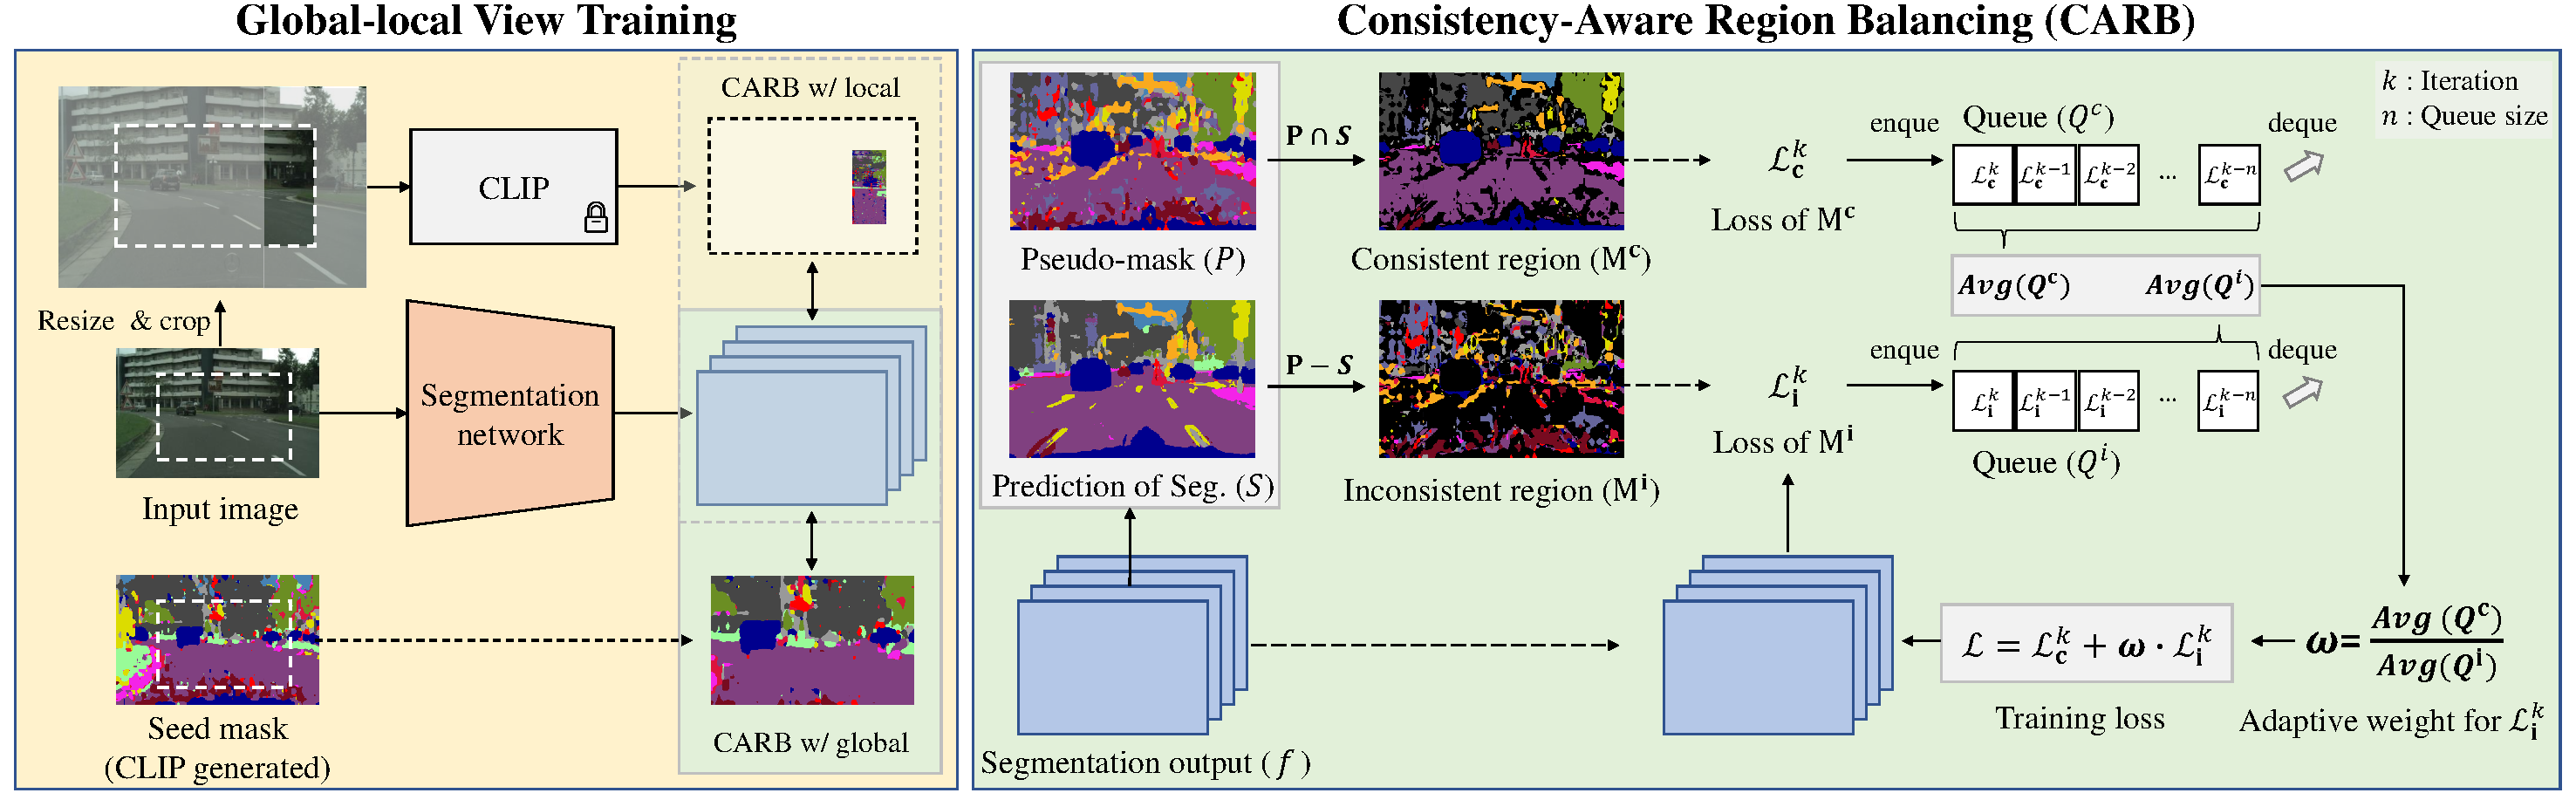
\includegraphics[width=17cm]{figures/fig_framework.pdf}
\caption{Overall framework of proposed method. (Global-local View Training) CLIP gives different pseudo masks for cropping and resizing. (CARB) The pseudo-mask is divided into the consistent / inconsistent regions and the high loss of inconsistent regions is suppressed via adaptive region balancing.}
\label{fig:framework}
\end{figure*}

\subsubsection{Uncertainty Estimation.} Estimating the uncertainty~\cite{DBLP:conf/nips/KendallG17} has been discussed in deep learning since deep neural networks learn to approximate probabilistic models. Focusing on semantic segmentation, the \citeauthor{feng2022dmt} utilizes an ensemble of models that are initialized differently to separate the uncertainty region. In a similar vein, several methods~\cite{oh2021background,DBLP:conf/aaai/ZhangXWSH20} utilized a combination of confidence thresholding and consistency between the CRF-refined mask and the original mask to define a reliable region. ST++~\cite{yang2022st++} identifies reliable images by utilizing the results of previous checkpoints. Recently, several methods suggest pixel-level entropy to measure the pixel-level uncertainty~\cite{NEURIPS2020_f73b76ce,Huynh:CVPR22,li2022uncertainty, wang2022semi}.

\section{Statistics of Datasets}
In this section, to identify the cause of the poor performance of existing WSSS methods on driving scenes, we compare the characteristics of two types of datasets: standard benchmark datasets (\eg, PASCAL VOC and MS COCO) and driving scene datasets (\eg, Cityscapes and CamVid). Specifically, we investigate the histograms of 1) the number of classes per image, 2) the co-occurrence ratio between classes, and 3) the number of positive/negative samples per class (Fig.~\ref{fig:dataset}).

The distinct difference between the two types of datasets is the number of classes in a single image. Although existing benchmark datasets have only one or two classes in most images, driving scene datasets typically contain eight or more classes in a single image, as in Fig.~\ref{fig:dataset}~(a). Next, we calculate the frequency ratio of co-occurrence between every pair of classes and plot a histogram of those ratios in Fig.~\ref{fig:dataset}~(b). Even worse, these classes in driving scenes often appear together, causing contextual bias. It is clearly different from PASCAL VOC and MS COCO.

Another critical point is the scarcity of negative samples in driving scene datasets. Negative samples are important learning signals for training the image classifier. As shown in Fig.~\ref{fig:dataset}~(c), existing datasets have a sufficient number of negative samples, but some classes in driving scene datasets have extremely few or zero negative samples. Most seriously, \textit{road} and \textit{car} in CamVid always appear in all training images and cannot be distinguished using only image-level labels. Understanding these characteristics is essential for developing productive approaches for WSSS using image-level labels in driving scene applications.

\begin{figure}[t]
\begin{center}
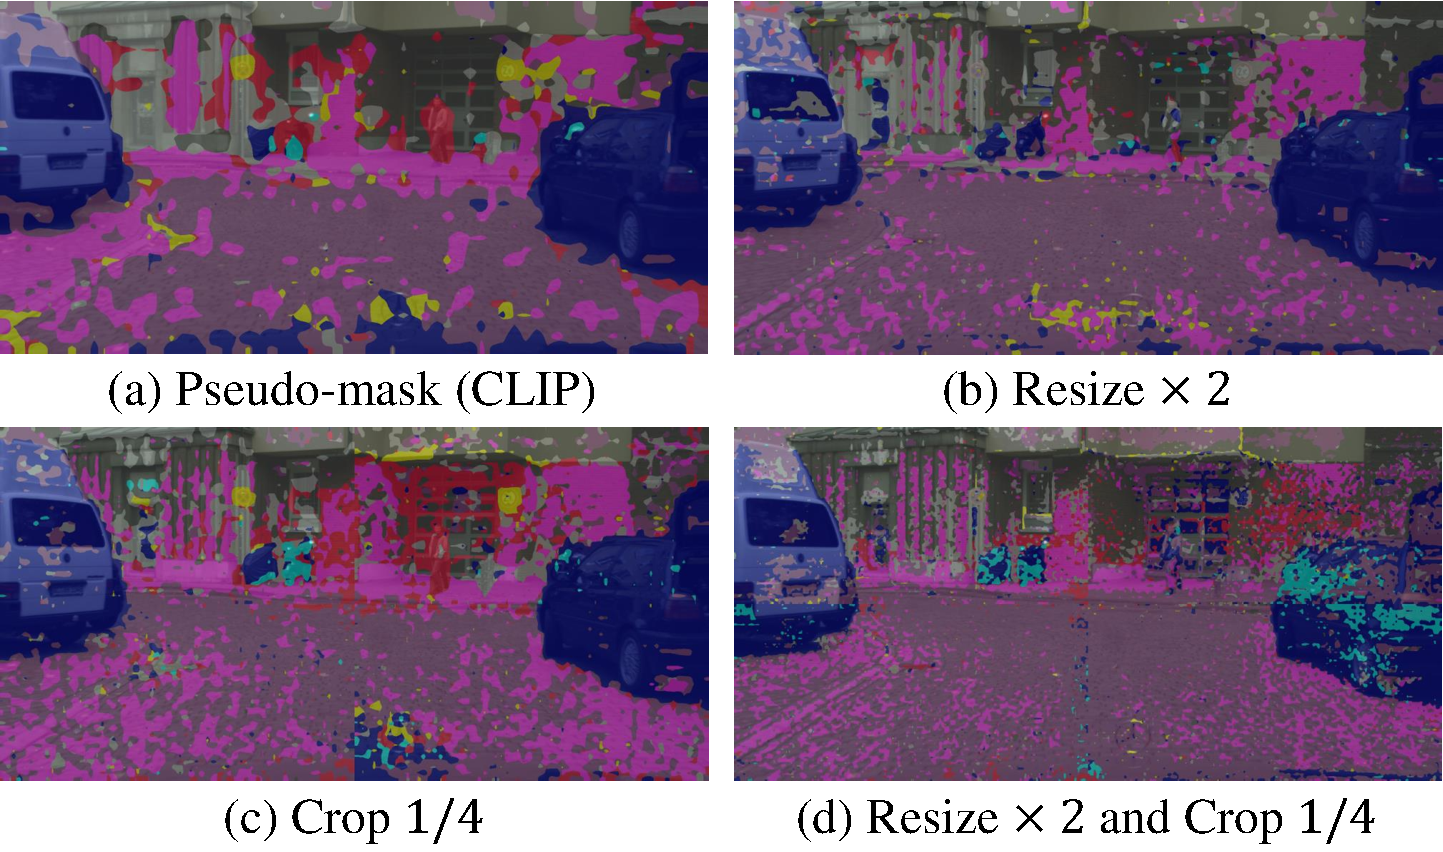
\includegraphics[width=8cm]{figures/fig_mask_resizencrop.pdf}
\end{center}
\caption{Pseudo-masks after resizing and cropping. (a) The original CLIP mask. (b) CLIP mask with resize ratio 2. (c) The concatenation of quarter-size cropped CLIP masks (d) The mask applying both operations. For visual clarity, we modify color palette of motorcycle to \textit{cyan} in this figure.}
\label{fig:mask_resizencrop}
\end{figure}

\begin{figure}[t]
\begin{center}
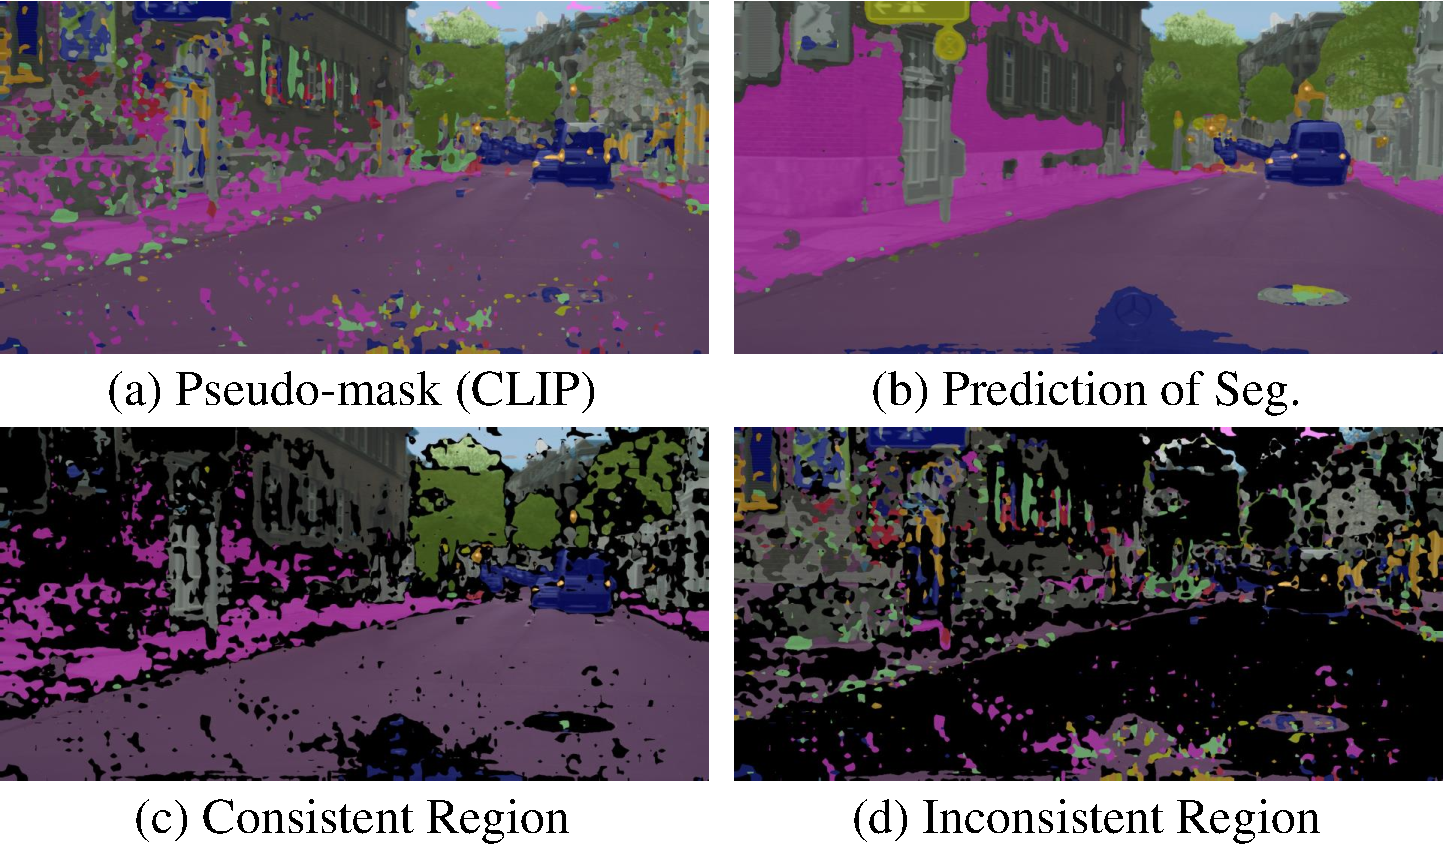
\includegraphics[width=8cm]{figures/fig_mask_character.pdf}
\end{center}
\caption{The characteristics of two different masks. (a) The mask from CLIP contains small and blob-like noisy regions. (b) The output mask from the segmentation network is more systematic. We identify reliable regions (c) based on prediction consistency between (a) and (b).}
\label{fig:mask_character}
\end{figure}

\begin{figure}[t]
\begin{center}
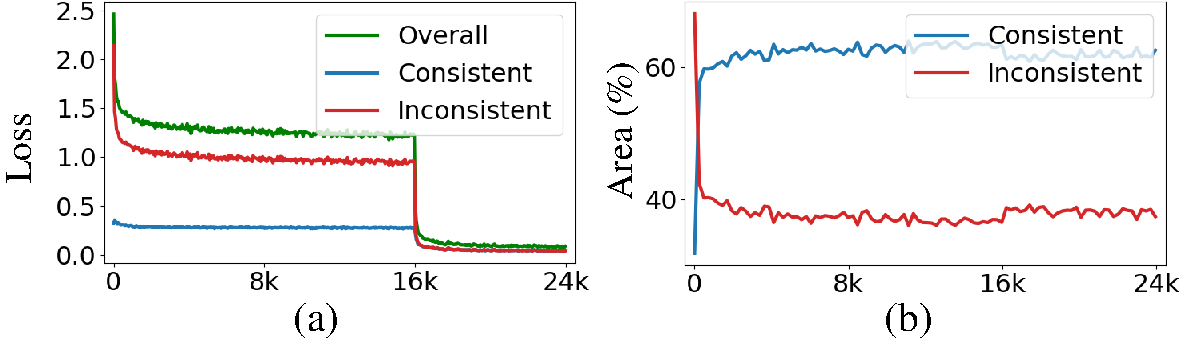
\includegraphics[width=\linewidth]{figures/fig_loss1.pdf}
\end{center}
\caption{Changes in (a) loss and (b) area of consistent/inconsistent regions during training. Adaptive region balancing is applied from 16K iteration, affecting the training dynamics.}
\label{fig:fig_loss1}
\end{figure}

\section{Method}

\subsection{Global-local View Training}
Owing to the specific nature of driving scenes, certain classes such as \textit{roads} are consistently large, and others like \textit{traffic light} remain small in size. Since the driving scenes capture road environments with a wide range of depth in each image, object sizes vary significantly with distance even within the same class, such as \textit{car}. In Fig.~\ref{fig:mask_resizencrop}~(a), we observe that the pseudo-masks generated by the CLIP model exhibit notably high quality for relatively large objects but poor quality for small objects. We conjecture that this performance degradation may occur from the training mechanism of CLIP (\ie, it mainly concentrate on salient objects corresponding to text prompt rather than small objects).

Building upon this observation, we manipulate the relative object size within the input by adjusting the \emph{image scale} and \emph{field-of-view} (FOV). We then analyze the resultant changes in the pseudo-mask obtained from CLIP. In Fig.~\ref{fig:mask_resizencrop}~(b), when the input is scaled to twice its original size, the pseudo-mask exhibit more accurate and fine-grained results along the object boundaries. Additionally, reducing the FOV by half (\ie, the network only observes one-quarter of the input at a time) leads to noticeable changes in the pseudo-mask, particularly pronounced for smaller objects such as \textit{motorcycle} (\cf, Fig~\ref{fig:mask_resizencrop}~(c)). This simple case study unveils distinctive characteristics associated with each adjustment.

Summarizing, we observed distinct responses of CLIP to cropping (changing FOV) and resizing (changing scales). (1) Resizing improves the localization at fine-grained areas such as edges. (2) Cropping enhances the classification of small objects. Capitalizing on the distinctive effects of cropping and resizing, we synergistically incorporate both augmentations into our approach. By jointly leveraging these functions, we enhance pseudo-mask performance, particularly for small objects.

Inspired by this observation, we have developed a new method called \textit{Local View Sampling}. This technique leverages the conventional augmented input known as the global view, commonly used for training segmentation networks. We extract a patch of a specific size (typically small) from an arbitrary position inside the global view. Then, the patch is resized randomly before passing it through CLIP. We obtain the local pseudo-mask by calculating the similarity of local features from the image encoder and text embedding as follows:

\begin{equation}
\label{eq_local_mask}
{\small
\mathbf{M}^\mathbf{l} = \arg \max(\frac{\boldsymbol{F}^\mathbf{l} \cdot \boldsymbol{t}}{\left \| \boldsymbol{F}^\mathbf{l} \right \| \cdot \left \| \boldsymbol{t} \right \|}),
}
\end{equation} %
%
where $\boldsymbol{F}^\mathbf{l}$ is the feature from CLIP with a local view image, $\boldsymbol{t}$ is text embedding of CLIP. The local view only contains semantic information in a small, confined, area, so it can fully exploit locality from CLIP. This empowers the pseudo-mask of the local view to better focus on small objects. We leverage the masks of both views to train the segmentation model. The loss for the global-local view training is computed by cross-entropy loss for each region as follows:
\begin{equation}
\label{eq_loss_loc}
{\small
\mathcal{L}_\mathbf{l} = - \frac{1}{|\mathbf{M}^\mathbf{l}|} \underset{i,j \in local}{\sum} \text{ } y^\mathbf{l} \log {f_{i,j}},
}
\end{equation}

\begin{equation}
\label{eq_loss_glo}
{\small
\mathcal{L}_\mathbf{g} = - \frac{1}{|\mathbf{M}^\mathbf{g}|} \underset{i,j}{\sum} \text{ } y^\mathbf{g} \log {f_{i,j}},
}
\end{equation}%
%
where $y^\mathbf{l}$ and $y^\mathbf{g}$ are one-hot labels of  $\mathbf{M}^\mathbf{l}$ and $\mathbf{M}^\mathbf{g}$, respectively. $\mathbf{M}^\mathbf{g}$ and $\mathbf{M}^\mathbf{l}$ are the global pseudo-mask and the local pseudo-mask, respectively. $f \in \mathbb{R}^{C \times H \times W}$ is the probability of segmentation network. The total loss for the global-local view training is $\mathcal{L} = \mathcal{L}_\mathbf{g} + \mathcal{L}_\mathbf{l}$.

\subsection{Consistency-aware Region Balancing} \label{sec:separation}
We identify noisy regions in the pseudo-mask created by CLIP. Fig.~\ref{fig:mask_character} showcases an example of a pseudo-mask containing small and blob-like noisy regions, randomly scattered on the image.

Conversely, training a segmentation network with pseudo-masks removes the randomly scattered noise of CLIP's pseudo-mask in the output, resulting in systematic predictions. (\eg, \textit{road} in Fig.~\ref{fig:mask_character} (b)) However, the segmentation prediction has misclassified pixels that were originally correct in the pseudo-mask. In particular, we observe that the trained segmentation model produces an indistinct boundary of the object even worse than the pseudo-mask generated by CLIP (\eg, \textit{sidewalk} in Fig.~\ref{fig:mask_character} (b)).

Owing to the unique properties of the trained segmentation model and CLIP, we leverage both models to benefit from their respective advantages. However, since the prediction of the segmentation model is already incorporated in the model, directly computing the loss using the segmentation prediction does not provide new evidence for training. To address this, we indirectly employ the segmentation prediction to distinguish the pixels of the pseudo-mask from CLIP. Specifically, utilizing prediction consistency, we regard the pixel as reliable if they are consistent and noisy if the predictions from the two models are inconsistent:

\begin{equation}
\label{eq_region_con}
{\small
\mathbf{M}^\mathbf{c} = \{P_{i,j} | P_{i,j} = S_{i,j}\},
}
\end{equation}
\begin{equation}
\label{eq_region_inc}
{\small
\mathbf{M}^\mathbf{i} = \{P_{i,j} | P_{i,j} \neq S_{i,j}\},
}
\end{equation}%
%
where $\mathbf{M}^\mathbf{c}$ and $\mathbf{M}^\mathbf{i}$ correspond to consistent and inconsistent regions, respectively. $P \in C^{H \times W}$ and $S \in C^{H \times W}$ are the pseudo-mask from CLIP and the prediction of the segmentation network, where $C$ is a set of classes. Furthermore, we apply label filtering when generating $S$ to prevent misprediction with non-existent classes in the image.

The consistent and inconsistent regions are recalculated in each iteration to update the segmentation model. As training progresses, we notice that the size of the consistent region changes, resulting in performance improvement of the segmentation model (Fig.~\ref{fig:fig_loss1}~(b)).

To understand the effects of consistent and inconsistent regions, we separately calculate the cross-entropy loss of each side:
\begin{equation}
\label{eq_loss_con}
{\small
\mathcal{L}_\mathbf{c} = - \frac{1}{|\mathbf{M}^\mathbf{c}|} \underset{i,j}{\sum} \text{ } y^\mathbf{c} \log {f_{i,j}},
}
\end{equation}

\begin{equation}
\label{eq_loss_inc}
{\small
\mathcal{L}_\mathbf{i} = - \frac{1}{|\mathbf{M}^\mathbf{i}|} \underset{i,j}{\sum} \text{ } y^\mathbf{i} \log {f_{i,j}},
}
\end{equation}%
%
where $y^\mathbf{c}$ and $y^\mathbf{i}$ are one-hot labels of  $\mathbf{M}^\mathbf{c}$ and $\mathbf{M}^\mathbf{i}$, respectively. $f \in \mathbb{R}^{C \times H \times W}$ is the probability of segmentation network. We observe that inconsistent regions have much higher loss values than consistent regions in Fig.~\ref{fig:fig_loss1} (a). If we treat the training loss equally across all regions, the network is overly influenced by the high loss produced from the inconsistent regions. Therefore, we suggest assigning different weights to the losses of consistent and inconsistent regions while taking into account the noise level of the data. It helps prevent the conventional cross-entropy loss from being vulnerable to noise in the training data.

To this end, we devise an adaptive region balancing method that dynamically adjusts the loss of the inconsistent region by monitoring the loss profiles in both the consistent and inconsistent regions during training. Specifically, we introduce two fixed-size queues which track the losses of the two regions, denoted as $\mathcal{L}_\mathbf{c}$ and $\mathcal{L}_\mathbf{i}$, respectively. We then compute the average loss from each queue. We use the ratio of two average losses as the weight for the cross-entropy loss of the inconsistent region, denoted as $w$, which is multiplied by the loss of the inconsistent region. The CARB training loss is $\mathcal{L} = \mathcal{L}_\mathbf{c} + w \cdot \mathcal{L}_\mathbf{i}$. This balancing ensures that the training is less influenced by the inconsistent region.

While one might consider that the loss from inconsistent regions can be simply neglected, our observations reveal that the inconsistent regions still possess useful learning signals. Notably, we observe that labels of highly correlated object classes (\ie, the classes sharing visual properties like \textit{bus} and \textit{car}) exist within the inconsistent region. Overlooking those pixels impedes the label imbalance problem. The Cityscapes dataset, for instance, includes classes like \textit{rider} (a subset of \textit{person}), \textit{bus}, and \textit{truck} (subsets of \textit{car}) that are susceptible to such confusion. Considering these challenges, we present a region-balancing method designed to harness meaningful information even from inconsistent regions.

\subsubsection{Overall Training.}
The proposed method consists of two stages. In the first stage, we warm up the baseline segmentation model with global and local views generated from CLIP masks. This step ensures that the segmentation network sufficiently learns the regular patterns of the target dataset. In the second stage, we refine the segmentation network utilizing CARB. We apply CARB for both global and local views.

\section{Experiments}
\subsection{Experimental Setup}
\subsubsection{Dataset \& Evaluation Metric.} For performance evaluation, we utilized the well-known Cityscapes~\cite{cordts2016cityscapes}, CamVid~\cite{brostow2009semantic}, and WildDash2~\cite{Zendel_2022_CVPR}, which are autonomous driving datasets. The Cityscapes dataset consists of 2,975 training, 500 validation, and 1,525 test images with fine annotation. It contains a total of 30 classes, and 19 classes are evaluated for public assessment while the rest are void. The CamVid dataset consists of 367 training, 101 validation, and 233 test images, containing a total of 32 classes. In our experiments, only 11 classes are evaluated by following the convention of previous research~\cite{wang2020deep}. The WildDash2 dataset consist of 3,618 training, 638 validation, and 812 test images, containing a total of 25 classes. In all experiments, we solely utilized image-level labels for training. The image-level labels are acquired from pixel-level labels of each dataset. Mean Intersection over Union (mIoU) was used as the evaluation criterion, a popular and standard metric for semantic segmentation.

\subsubsection{Implementation Detail.}
We employed ViT-B/16~\cite{dosovitskiyimage} as the image encoder for the CLIP, and ResNet50~\cite{he2016deep}-based DeepLab-ASPP~\cite{chen2017deeplab} as the segmentation network. The last convolutional layer of ASPP was replaced with text embedding of CLIP. The segmentation network was initialized with an ImageNet pre-trained model provided by MMSeg~\cite{mmseg2020}. Considering class definition and object words connoting actual objects, we replaced the \textit{vegetation} and \textit{terrain} class names with \textit{tree} and \textit{grass}, respectively. Furthermore, we changed the \textit{person} class to \textit{pedestrian}, since it is a superset of the \textit{rider}. For generating pseudo-masks from CLIP, we adopt MaskCLIP~\cite{zhou2022extract}.

\begin{table}[]
\normalsize
\centering
{\small
\begin{tabular}{@{}lc@{}}
\toprule
Method          & \multicolumn{1}{c}{mIoU}  \\ \midrule
Base                                & \multicolumn{1}{c}{40.1} \\
\multicolumn{1}{l}{+ CARB}           & \multicolumn{1}{c}{45.7} \\
\multicolumn{1}{l}{+ Local}          & \multicolumn{1}{c}{45.1} \\
\multicolumn{1}{l}{+ Local + CARB}   & \multicolumn{1}{c}{50.6} \\
\multicolumn{1}{l}{+ Dual}           & \multicolumn{1}{c}{45.8} \\
\multicolumn{1}{l}{+ Dual + CARB}    & \multicolumn{1}{c}{\textbf{52.1}} \\

\bottomrule
\end{tabular}
}
\caption{Ablation study of the proposed modules. The accuracy (mIoU) is evaluated on the Cityscapes validation set. The best score is in \textbf{bold} throughout all experiments.}
\label{tab:split}
\end{table}

\subsection{Ablation Study}
\label{sec:ablation}
\subsubsection{Effects of Each Module.} We evaluate the effectiveness of each component of our method in Tab.~\ref{tab:split}. When we train the segmentation model with additional local view sampling ($Local$), it shows a remarkable improvement of 5.0\%p. This implies that additional information from local patches through cropping and resizing provides rich learning signals. CARB alone contributed an impressive improvement of 5.6\%p, indicating that adaptively re-weighting the loss according to its reliability plays a critical role in learning with noisy pseudo-masks. By combining local view sampling and CARB ($Local + CARB$), a substantial improvement of 10.5\%p was achieved. Instead of $Local$, we added a slight modification named $Dual$, by re-creating the mask of global views depending on the augmentation using CLIP for each iteration. This modification yielded a 0.7\%p gain over $Local$. Interestingly, our $Dual+CARB$ method shows a 1.5\%p improvement compared to $Local + CARB$, indicating synergy between various-sized mask creations and our noise-handling strategy.

\begin{figure}[t]
\begin{center}
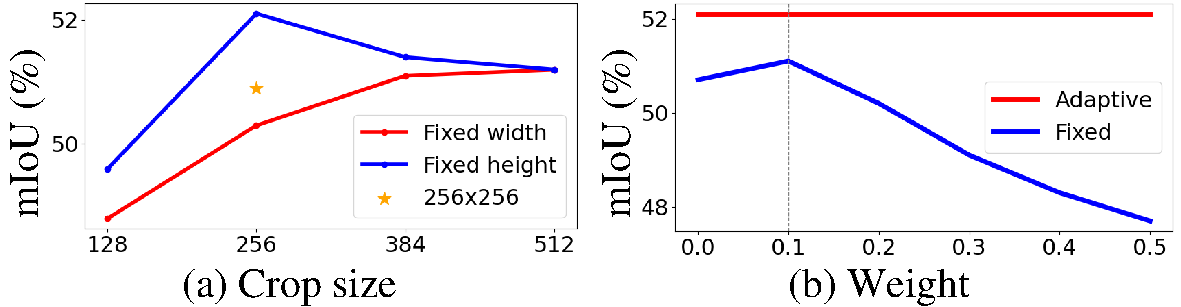
\includegraphics[width=\linewidth]{figures/fig_ablation.pdf}
\end{center}
\caption{Segmentation results (mIoU) on Cityscapes validation set depending on (a) the crop size (b) the weight. We set the length of one side to 512 and varied the length of the other side between 128 and 512. Yellow star indicates the experiment using $256 \times 256$ patch.}
\label{fig:ablation}
\end{figure}

\begin{table}[]
\normalsize
\centering
{\small
\begin{tabular}{@{}lrr@{}}
\toprule
\multicolumn{1}{c}{Method}                              & \multicolumn{1}{c}{val} & \multicolumn{1}{c}{test} \\ \midrule
\multicolumn{1}{l}{DeepLab-ASPP (Full supervision)} & 78.3 & \multicolumn{1}{r}{75.8} \\ \midrule
\multicolumn{1}{l}{AffinityNet} &  8.2 & \multicolumn{1}{r}{-} \\
\multicolumn{1}{l}{SEAM} & 17.3 & \multicolumn{1}{r}{-} \\
\multicolumn{1}{l}{1-Stage} & 11.8 & \multicolumn{1}{r}{-} \\
\multicolumn{1}{l}{\citeauthor{wang2020deep}} & 24.2 & \multicolumn{1}{r}{24.9}          \\
\multicolumn{1}{l}{CAM} & 33.0 & \multicolumn{1}{r}{32.2} \\
% \multicolumn{1}{l}{EPS} & 29.4 & \multicolumn{1}{r}{28.6} \\
\multicolumn{1}{l}{AMN} & 17.5 & \multicolumn{1}{r}{17.8} \\
\multicolumn{1}{l}{CLIMS } & 18.1 & \multicolumn{1}{r}{18.0} \\
\multicolumn{1}{l}{CLIP-ES } & 35.4 & \multicolumn{1}{r}{35.0} \\ \midrule
\multicolumn{1}{l}{Ours}                                & \textbf{52.1}     & \multicolumn{1}{r}{\textbf{51.8}} \\ \bottomrule

\end{tabular}
}
\caption{Segmentation results (mIoU) on Cityscapes.}
\label{tab:seg_cityscapes}
\end{table}

\subsubsection{Effects of the Crop Size and Resize Ratio.} In our empirical investigation, it was consistently observed that vertically long rectangular patches exhibited superior performance in terms of crop sizes compared to patches of other sizes. This finding is supported by Fig.~\ref{fig:ablation}. We conjecture this tendency in the driving scene dataset comes from vertically long structures such as \textit{pole} and \textit{traffic light}. Also, the 512$\times$512 patches for local views are more effective than the 256$\times$256. These experiments suggest that, while the local view represents a smaller portion of the overall scene, excessively small sizes may not benefit from the attention layers equipped in CLIP.

We evaluated our local view sampling under variable resize ratios. Under the fixed ratio from 0.5 to 2.0, we observe the best performance of 52.1\% at the ratio of 1.0 while a significant drop with other ratios. However, when focusing on classwise performances under various resize ratios, we confirmed that a large resize rate benefits the performance of small classes, such as \textit{traffic light} and \textit{rider}. Meanwhile, the performance of the large classes, such as \textit{sidewalk} and \textit{wall}, is decreased. Due to the performance trade-off across different classes, we set a random value between 1.0 and 2.0 as the resize ratio. Our choice leads to the overall best performance in both small and large classes.

\subsubsection{Effects of Adaptive Region Balancing.} We compare our adaptive region balancing strategy with a fixed weighting strategy, where the loss weight for the inconsistent region ($w$) is set to a specific value (\cf, Fig.~\ref{fig:ablation} (b)). When changing the fixed weight $w$ gradually from 0 to 0.5, we observe the best score at the weight of 0.1 and a significant drop with other values. Although the highest performance of the fixed weight strategy is similar to that of our method (51.06\% for fixed strategy and 52.1\% for our method), it requires a hyperparameter search for the optimal weight using the validation dataset. In contrast, our method does not require such a search, making it more suitable for WSSS scenario.

\subsection{Quantitative Comparisons}
\subsubsection{Remarks on Comparisons.} Existing WSSS methods focus on handling object-centric datasets such as PASCAL VOC 2012. Therefore, their methods are primarily designed to distinguish relatively simple object shapes with similar scales, which is still a valuable research direction. Given this dataset mismatch, direct comparisons between our method and existing WSSS approaches might not be entirely fair, as they cater to distinct dataset characteristics. Nevertheless, by adapting established WSSS methods to driving scenes, we intend to show that the existing framework is ineffective for our application scenario.

\begin{figure*}[t!]
\centering
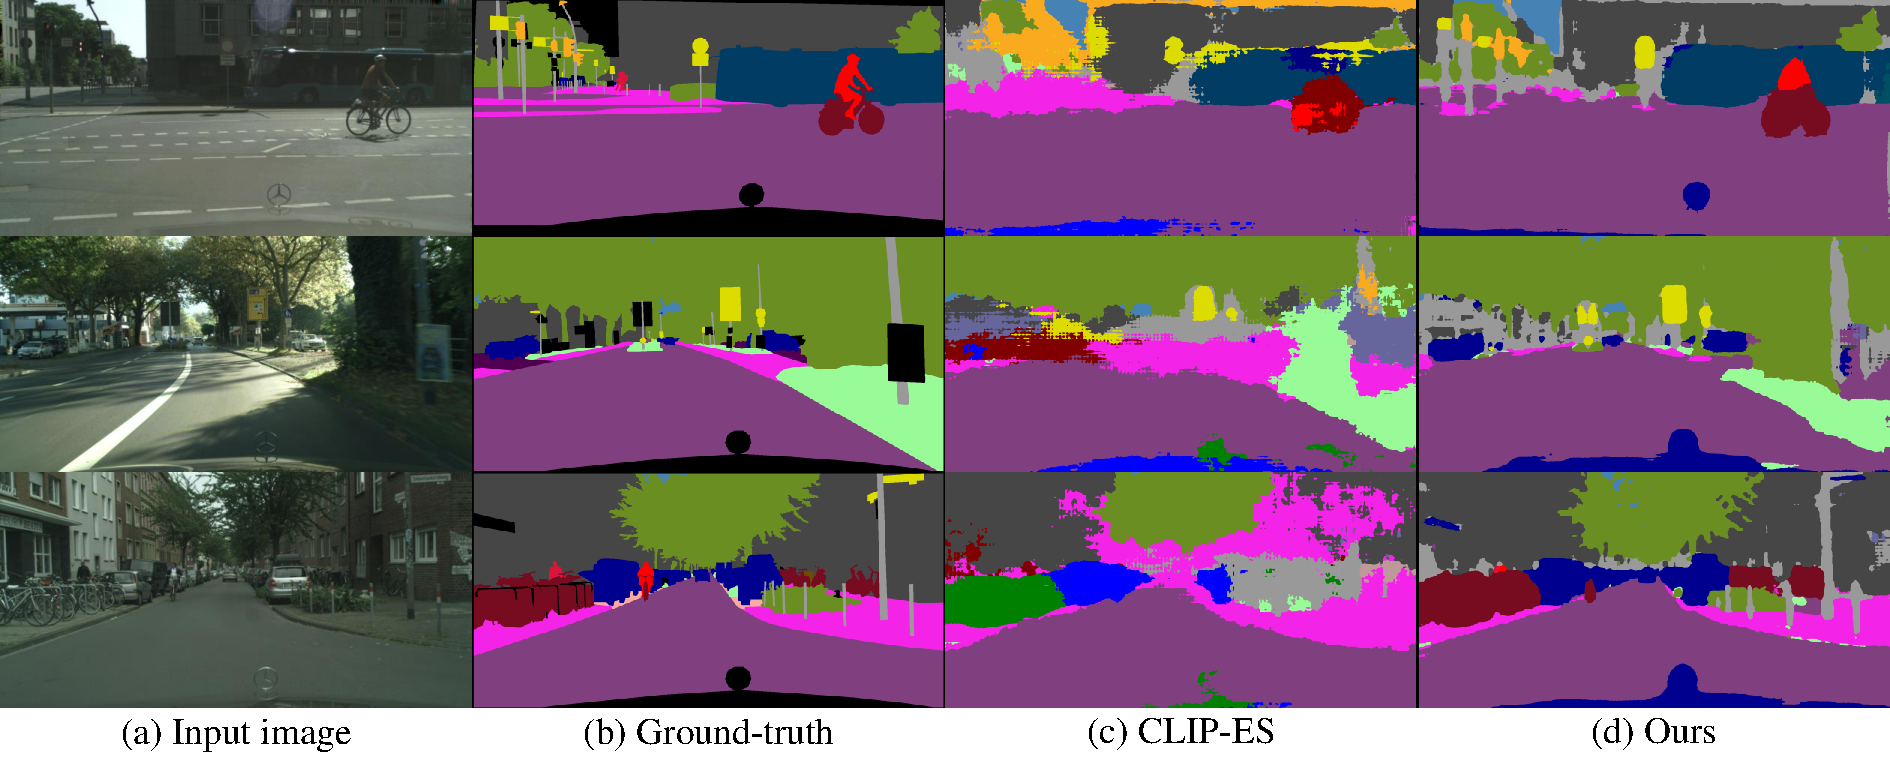
\includegraphics[width=16cm]{figures/fig_qualitative_city.pdf}
\caption{Qualitative results on Cityscapes validation set. (a) Input image, (b) Ground-truth, (c) CLIP-ES, and (d) Our method.}
\label{fig:qualitative_city}
\end{figure*}

\subsubsection{Existing WSSS Methods.} Existing methods can be partitioned into CAM-based methods (\ie, an image classifier for generating the pseudo-masks) and CLIP-based methods (\ie, CLIP for generating the pseudo-masks). Among them, we choose several representative methods such as (1) AffinityNet~\cite{ahn2018learning}, (2) SEAM~\cite{wang2020self}, (3) 1-Stage~\cite{araslanov2020single}, (4) SEC~\cite{kolesnikov2016seed}, (5) Wang et al.~\cite{wang2020deep}, (6) CAM~\cite{zhou2016learning}, and  (7) AMN~\cite{lee2022threshold}. To compare with CLIP-based WSSS, we reproduce the driving scene results of (8) CLIMS~\cite{Xie_2022_CVPR} and (9) CLIP-ES~\cite{Lin_2023_CVPR}, both of which use the same level of information, CLIP, as our method.

\begin{table}[]
\normalsize
\centering
{\small
\begin{tabular}{@{}lrr@{}}
\toprule
\multicolumn{1}{c}{Method}          & \multicolumn{1}{c}{val}   & \multicolumn{1}{c}{test} \\ \midrule
\multicolumn{1}{l}{DeepLab-ASPP (Full supervision)}     & 81.6                      & \multicolumn{1}{r}{74.9}              \\ \midrule
\multicolumn{1}{l}{SEC} & - &  \multicolumn{1}{r}{2.5}              \\
\multicolumn{1}{l}{AffinityNet} & 11.0 & \multicolumn{1}{r}{15.5} \\
\multicolumn{1}{l}{\citeauthor{wang2020deep}} & 23.5 & \multicolumn{1}{r}{30.4} \\
\multicolumn{1}{l}{CAM} & 9.6 & \multicolumn{1}{r}{6.6} \\
\multicolumn{1}{l}{AMN} & 10.7 & \multicolumn{1}{r}{7.6} \\
\multicolumn{1}{l}{CLIMS} & 2.7 & \multicolumn{1}{r}{4.3} \\
\multicolumn{1}{l}{CLIP-ES} & 41.7 & \multicolumn{1}{r}{39.6} \\ \midrule
\multicolumn{1}{l}{Ours} & \textbf{55.7} & \multicolumn{1}{r}{\textbf{50.5}} \\ \bottomrule
\end{tabular}
}

\caption{Segmentation results (mIoU) on CamVid.}
\label{tab:seg_camvid}
\end{table}

\subsubsection{Cityscapes.} Tab.~\ref{tab:seg_cityscapes} presents the performance of our proposed CARB compared to other methods in driving scenes. Specifically, our approach achieves 51.8\% on the Cityscapes test set, which outperforms the \citeauthor{wang2020deep} by 26.9\%p and
previous CLIP-based WSSS technique by 16.8\%p. Additionally, we observed that our method consistently performs better than CLIP-ES in every class. Fig.~\ref{fig:qualitative_city} showcases qualitative examples of segmentation results on the Cityscapes. Notably, CARB successfully eliminates misclassified \textit{sidewalk} regions on the \textit{sky} class (see the first and second rows). These results visually confirm that our method correctly captures each class and successfully reduces the prediction errors.

\subsubsection{CamVid.} The CamVid dataset has a much smaller number of training images compared to Cityscapes, with only 367 images. Additionally, it is not possible to differentiate between the \textit{car} and \textit{road} classes using only image-level labels, as they appear in all images. However, our method can distinguish them by utilizing the pre-trained image-text information from the CLIP model. Tab.~\ref{tab:seg_camvid} shows that the performance of CAM-based methods (\eg, SEC, AffinityNet, \citeauthor{wang2020deep}, and CLIMS) is considerably low while our method achieves significantly higher performance. This demonstrates that our proposed approach can address the problem even when the scale of the dataset is small and has severe contextual bias. %(\ie, classes are indistinguishable only with image-level labels).

\subsubsection{WildDash2.} Since the WildDash2 dataset possesses extremely high diversity, it is generally challenging even for the fully supervised model. A classifier-based WSSS method such as CLIMS performs poorly, 1\% in mIoU, which is worse than a random guess. This poor performance is caused by difficulties in training the classifier due to class imbalance and complex class distribution. Since CLIP-ES and our method are built upon CLIP for generating the pseudo masks, both methods provide relatively reasonable performances. Our method achieves considerably high performance compared to CLIP-ES, with the performance gain primarily observed in small classes such as \textit{billboard}, \textit{rider}, \textit{bicycle}, and \textit{road marking}.

\begin{table}[]
\centering
{\small
\begin{tabular}{@{}lr@{}}
\toprule
\multicolumn{1}{c}{Method}                              & \multicolumn{1}{c}{Result} \\ \midrule
\multicolumn{1}{l}{DeepLab-ASPP (Full supervision)}     & \multicolumn{1}{r}{54.0}          \\ \midrule
\multicolumn{1}{l}{CAM} & \multicolumn{1}{r}{15.2} \\
\multicolumn{1}{l}{AMN} & \multicolumn{1}{r}{18.8} \\
\multicolumn{1}{l}{CLIMS} & \multicolumn{1}{r}{1.0} \\
\multicolumn{1}{l}{CLIP-ES} & \multicolumn{1}{r}{24.7}          \\ \midrule
\multicolumn{1}{l}{Ours}                                & \multicolumn{1}{r}{\textbf{32.2}} \\ \bottomrule
\end{tabular}
}
\caption{Segmentation results (mIoU) on WildDash2 \textit{val} set.}
\label{tab:seg_coarse}
\end{table}

\section{Conclusion}
This paper addressed the limitations of conventional CAM-based, weakly-supervised semantic segmentation (WSSS) methods when handling the driving scene datasets. To break the performance bottleneck of the CAM-based methods, we utilized CLIP as the pseudo-mask generator. Then, we proposed global-local view training, which exploits the characteristics of CLIP generating diverse masks depending on the relative object sizes. We also propose a novel training strategy, namely consistency-aware region balancing (CARB). It distinguishes between reliable and noisy regions utilizing prediction consistency and then suppresses the latter regions during training. By incorporating  these two components, our method successfully (1) learns to segment small objects and (2) heavily relies on reliable regions while effectively handling challenging objects from noisy regions. Extensive experiments demonstrate that each component of our method contributes to achieving new state-of-the-art performances on the Cityscapes, CamVid, and WildDash2 datasets in WSSS. Our study introduces a new approach addressing the challenges posed by driving datasets and suggests a promising direction for future research in WSSS.

\section*{Acknowledgments}
This research was supported by the Basic Science Research Program through the National Research Foundation of Korea (NRF) funded by the MSIP (NRF-2022R1A2C3011154, RS-2023-00219019, RS-2023-00240135) and MOE (NRF-2022R1A6A3A13073319), the IITP grant funded by the Korea government(MSIT) (No. 2019-0-00075, Artificial Intelligence Graduate School Program(KAIST)), KEIT grant funded by the Korea government(MOTIE) (No. 2022-0-00680, 2022-0-01045, 2021-0-02068, Artificial Intelligence Innovation Hub) and Samsung Electronics Co., Ltd (IO230508-06190-01).

%File: anonymous-submission-latex-2023.tex
\documentclass[letterpaper]{article} % DO NOT CHANGE THIS
\usepackage{aaai23}  % DO NOT CHANGE THIS
\usepackage{times}  % DO NOT CHANGE THIS
\usepackage{helvet}  % DO NOT CHANGE THIS
\usepackage{courier}  % DO NOT CHANGE THIS
\usepackage[hyphens]{url}  % DO NOT CHANGE THIS
\usepackage{graphicx} % DO NOT CHANGE THIS
\urlstyle{rm} % DO NOT CHANGE THIS
\def\UrlFont{\rm}  % DO NOT CHANGE THIS
\usepackage{natbib}  % DO NOT CHANGE THIS AND DO NOT ADD ANY OPTIONS TO IT
\usepackage{caption} % DO NOT CHANGE THIS AND DO NOT ADD ANY OPTIONS TO IT
\frenchspacing  % DO NOT CHANGE THIS
\setlength{\pdfpagewidth}{8.5in} % DO NOT CHANGE THIS
\setlength{\pdfpageheight}{11in} % DO NOT CHANGE THIS
%
% These are recommended to typeset algorithms but not required. See the subsubsection on algorithms. Remove them if you don't have algorithms in your paper.
% \usepackage{algorithm2e}
% \usepackage{algorithmic}

% Use the postscript times font!
\usepackage{times}
\usepackage{soul}
\usepackage{url}
\usepackage[utf8]{inputenc}
% \usepackage[small]{caption}
\usepackage{graphicx}
\usepackage{amsmath}
\usepackage{amsthm}
\usepackage{booktabs}
\usepackage{algorithm}
\usepackage{algorithmic}
\usepackage[algo2e,linesnumbered,ruled,vlined]{algorithm2e} 

\newenvironment{console}{\ttfamily}{\par}
\urlstyle{same}
\linespread{0.99}


\usepackage{amsmath,amssymb,amsfonts} % Added for HYDRA
\newcommand{\tuple}[1]{\ensuremath{\left \langle #1 \right \rangle }} % Added for HYDRA
\newcommand{\reals}{\ensuremath{\mathbb{R}}} % Added for HYDRA
\usepackage[obeyFinal,final]{todonotes} % Added for HYDRA
\usepackage{xspace} % Added for HYDRA
\newcommand{\sbirds}{Science Birds\xspace} % Added for HYDRA % TODO Replace with acronym
\newcommand{\hydra}{\textsc{Hydra}\xspace} % Added for HYDRA % TODO Replace with acronym

\newcommand{\simulate}{\textit{Simulate}\xspace} % 

\newcommand{\wiktor}[1]{{\textcolor{red}{[Wiktor: #1]}}}
\newcommand{\shiwali}[1]{{\textcolor{orange}{[Shiwali: #1]}}}
\newcommand{\roni}[1]{{\textcolor{green}{[Roni: #1]}}}

\newtheorem{example}{Example}
\newtheorem{theorem}{Theorem}
\newtheorem{definition}{Definition} % Added for HYDRA


%
% These are are recommended to typeset listings but not required. See the subsubsection on listing. Remove this block if you don't have listings in your paper.
\usepackage{newfloat}
\usepackage{listings}
\DeclareCaptionStyle{ruled}{labelfont=normalfont,labelsep=colon,strut=off} % DO NOT CHANGE THIS
\lstset{%
	basicstyle={\footnotesize\ttfamily},% footnotesize acceptable for monospace
	numbers=left,numberstyle=\footnotesize,xleftmargin=2em,% show line numbers, remove this entire line if you don't want the numbers.
	aboveskip=0pt,belowskip=0pt,%
	showstringspaces=false,tabsize=2,breaklines=true}
\floatstyle{ruled}
\newfloat{listing}{tb}{lst}{}
\floatname{listing}{Listing}
%
% Keep the \pdfinfo as shown here. There's no need
% for you to add the /Title and /Author tags.
\pdfinfo{
/TemplateVersion (2023.1)
}

% DISALLOWED PACKAGES
% \usepackage{authblk} -- This package is specifically forbidden
% \usepackage{balance} -- This package is specifically forbidden
% \usepackage{color (if used in text)
% \usepackage{CJK} -- This package is specifically forbidden
% \usepackage{float} -- This package is specifically forbidden
% \usepackage{flushend} -- This package is specifically forbidden
% \usepackage{fontenc} -- This package is specifically forbidden
% \usepackage{fullpage} -- This package is specifically forbidden
% \usepackage{geometry} -- This package is specifically forbidden
% \usepackage{grffile} -- This package is specifically forbidden
% \usepackage{hyperref} -- This package is specifically forbidden
% \usepackage{navigator} -- This package is specifically forbidden
% (or any other package that embeds links such as navigator or hyperref)
% \indentfirst} -- This package is specifically forbidden
% \layout} -- This package is specifically forbidden
% \multicol} -- This package is specifically forbidden
% \nameref} -- This package is specifically forbidden
% \usepackage{savetrees} -- This package is specifically forbidden
% \usepackage{setspace} -- This package is specifically forbidden
% \usepackage{stfloats} -- This package is specifically forbidden
% \usepackage{tabu} -- This package is specifically forbidden
% \usepackage{titlesec} -- This package is specifically forbidden
% \usepackage{tocbibind} -- This package is specifically forbidden
% \usepackage{ulem} -- This package is specifically forbidden
% \usepackage{wrapfig} -- This package is specifically forbidden
% DISALLOWED COMMANDS
% \nocopyright -- Your paper will not be published if you use this command
% \addtolength -- This command may not be used
% \balance -- This command may not be used
% \baselinestretch -- Your paper will not be published if you use this command
% \clearpage -- No page breaks of any kind may be used for the final version of your paper
% \columnsep -- This command may not be used
% \newpage -- No page breaks of any kind may be used for the final version of your paper
% \pagebreak -- No page breaks of any kind may be used for the final version of your paperr
% \pagestyle -- This command may not be used
% \tiny -- This is not an acceptable font size.
% \vspace{- -- No negative value may be used in proximity of a caption, figure, table, section, subsection, subsubsection, or reference
% \vskip{- -- No negative value may be used to alter spacing above or below a caption, figure, table, section, subsection, subsubsection, or reference

\setcounter{secnumdepth}{0} %May be changed to 1 or 2 if section numbers are desired.

% The file aaai23.sty is the style file for AAAI Press
% proceedings, working notes, and technical reports.

% Title
\title{Domain-Independent Planning Model Repair via Heuristic Search}

% \iffalse
%Example, Multiple Authors, ->> remove \iffalse,\fi and place them surrounding AAAI title to use it
\author {
    % Authors
    Wiktor Piotrowski,\textsuperscript{\rm 1}
    Roni Stern, \textsuperscript{\rm 1,2}
    Yoni Sher, \textsuperscript{\rm 1}
    Jacob Le,\textsuperscript{\rm 1}
    Matthew Klenk, \textsuperscript{\rm 3}
    Johan de Kleer\textsuperscript{\rm 1}
    Shiwali Mohan,\textsuperscript{\rm 1}
}
\affiliations {
    % Affiliations
    \textsuperscript{\rm 1} Palo Alto Research Center, CA, USA\\
    \textsuperscript{\rm 2} Ben-Gurion University of the Negev, Beer-Sheva, Israel\\
    \textsuperscript{\rm 3} Toyota Research Institute, CA, USA\\
    wiktorpi@parc.com, sternron@post.bgu.ac.il, yonsher@parc.com, jale@parc.com, klenk.matthew@tri.global, dekleer@parc.com, smohan@parc.com
}
% \fi


\begin{document}

\maketitle

\begin{abstract}
Automated planning agents are largely ill-equipped to act in dynamic environments where a novelty can affect their fundamental characteristics and behavior. 
%Such scenarios are usually the domain of Reinforcement Learning agents. 
Model-based agents are often characterized by static planning models and rigid unchanging assumptions about the dynamic environments in which they operate. Contingency strategies, such as immediate replanning upon execution failure, only address a small fraction of cases and fail when it is unknown how the novelty has changed the environment. We propose a heuristic search-based domain-independent approach to simultaneously identify the novelty and repair the agent's planning model to adapt to the unexpected changes in its environment. We report empirical evaluations on the well-known balancing Cartpole problem, a standard Reinforcement Learning (RL) benchmark and Angry Birds, an established IJCAI competition domain. Our results show that by exploiting the proposed model repair approach, our PDDL+-based agents are able to quickly and effectively detect and adapt to some classes of novelties.
\end{abstract}

\section{Introduction}

% One hallmark of human cognition is our ability to function in an open world. People navigate to previously unseen places, perform new tasks, and integrate new technology into their lives. In dynamic environments, such as games, human flexibility supports inventing new strategies along with adapting to changing rules and shifting conditions. 

% On the other hand, learning-based agents are geared towards more dynamic environments where the agent's internal model is more fluid. However, while current AI systems can perform with superhuman capability in many closed-world game domains, even minor perturbations of the game can lead to significant drops in performance. 
% For example, Witty et al.~\shortcite{witty2018measuring} demonstrated that even changes which made the game easier could cause catastrophic results for superhuman-performing deep Q-learning agents without significant retraining.

%One hallmark of human cognition is our ability to function in an open, constantly evolving world. We navigate to previously unseen places, perform new tasks, and integrate new technology into our lives. While AI systems have made great strides in a variety of tasks including achieving super-human performance in several games such as Chess and Go, flexible reasoning \& learning in open worlds still remains a challenge. Despite a great variability in computational approaches, all AI systems are built with certain assumptions about the environment dynamics. These may be explicit as in model-based reasoning systems or may be implicit in the datasets over which learning systems are trained. It is inevitable that these assumptions are violated when the systems are fielded in real-world applicahttps://www.overleaf.com/project/62ead33f0d4b4929a13b0af4tions either because they were incorrectly determined or because the environment evolved. 

%In this paper, we study the problem of open-world learning \cite{senator2019sailon, langley2020open} - scenarios in which certain \emph{novelties} change the core dynamics of the environment suddenly while the agent is operational. 

Automated Planning strives to tackle complex problems rooted in real-world applications. However, model-based planning agents are largely ill-equipped to act in dynamic environments. Realistic scenarios include shifting conditions and unforeseen changes affecting the core characteristics of the environments. \citet{langley2020open} refers to such impactful changes as \emph{novelty}. In this paper, we focus on scenarios where a novelty can change the underlying model suddenly and at any time, in unknown and unexpected ways \emph{not according to the known system dynamics}. 

The vast majority of planning models, and particularly ones described in PDDL~\cite{mcdermott1998pddl} and its various levels, assume a static and deterministic world. They are rife with abstractions and approximations, and contain fixed values of important constants hand-selected by the designer. As a result, while planning models can capture the essence of a realistic scenario and offer explainability, they are often not sufficiently adaptable since the model can quickly fall out of alignment with the changing environment it is supposed to represent. Such inadequacies become apparent only after a plan has failed during its execution. Moreover, a failed plan execution does not identify the source of the issues, it merely notifies of an error or inaccuracy in the model. Unexpected changes in the latent part of the environment are notoriously difficult to detect and identify, and cannot be handled using conventional contingency acting strategies such as replanning~\cite{nebel1995plan}. 

Dynamic environments are often used as motivation for learning methods such as reinforcement learning (RL). RL makes minimal assumptions about the dynamics of the environment and uses feedback from the environment to learn action selection. While promising, RL methods have some significant shortcomings. \citet{witty2018measuring} studied deep Q-learning agents and demonstrated that even changes that make the task easier can lead catastrophic failures. Further, RL agents require large amounts of training experience that may not be accessible in real-world settings. And, finally, knowledge acquired by RL agents is distributed in a q-network or a q-table and is challenging to explain.  

%On the other hand, learning-based agents are geared towards more dynamic environments where the agent's internal model is more fluid. However, while current AI systems can perform with superhuman capability in many closed-world game domains, even minor perturbations of the game can lead to significant drops in performance. 
%For example, Witty et al.~\shortcite{witty2018measuring} demonstrated that even changes which made the game easier could cause catastrophic results for superhuman-performing deep Q-learning agents without significant retraining. 
%Despite the aforementioned shortcomings, model-based agents have the advantage of robustness over learning-based approaches. When sudden changes occur in the environment, normally, only a part of the agent's internal reasoning model requires updating. Still, adapting to novelty poses a major challenge in reliably deploying model-based agents in dynamical environments. 

% This mismatch between human cognitive abilities and machine capabilities indicates that effectively responding to novelty is a major problem in current AI systems~\cite{senator2019sailon}. 

Despite the aforementioned shortcomings of model-based planning, it is worthwhile to investigate approaches that adapt the model based on observations from the environment. Not only can planning models be robust to minor perturbations in the environment, adaptation to novelty usually requires changing only a small part of the model and can be done in a data-efficient manner. 

The main contribution of this paper is an \emph{domain-independent approach for adaptive repair of planning models}. Our approach can autonomously detect and characterize novelties introduced in the environment, as well as adapt the underlying planning model to the introduced novelty for robust behavior. The adaptation is performed via domain-independent heuristic search that generates modifications to the planning model that capture the effects of novelty on the environment. 
%The agent's internal model of the environment is modified via a mechanism that uses heuristic search to find a sequence of modifications to the model. The objective is for the modified model to capture the introduced novelty and once again accurately represent the changed execution environment. Accuracy of the agent's model is measured via the inconsistency score, checking for alignment between expectations (planned trace) and observations (execution trace). 
%The approach modifies the explicit planning model via a state-based search guided by a domain-independent heuristic measuring the consistency between predicted behavior and execution observations. 

Our approach is applicable to various levels of PDDL, though, we argue that representing meaningfully complex environments and novelties requires a highly expressive modeling language to capture their intricate structures and dynamics with sufficient accuracy. Our approach implemented in planning agents that reason over a PDDL+ model~\cite{fox2006modelling} of the environment to plan actions. 
We empirically evaluate the approach on a (RL) benchmark - OpenAI Gym's balancing Cartpole domain~\cite{barto1983neuronlike,brockman2016openai} and compare the results against deep-q network (DQN) RL agents. Our results show that model-based planning agents are \emph{resilient} to novelties; i.e, the degradation in their performance is not as severe as the DQN agent. Second, we show that our proposed approach enables a planning agent to adapt \emph{quickly}, requiring less than $20$ episodes to return to optimal performance after novelty has been introduced, much faster than the DQN RL agent. Finally, our approach is  \emph{explainable} by design. The adaptations are represented in terms of changes to the elements of its PDDL+ domain model enabling inspection of the proposed changes. 

In addition to being crucial for operations in dynamic environments with novelties, adaptive model repair is a versatile mechanism that can be exploited in various ways. It can be used improve the planning model accuracy by adjusting the values of the environment's parameters and variables based on observations made during plan execution. We report empirical results from AngryBirds, an IJCAI competition domain to demonstrate this capability.


%It is challenging to write accurate planning models and often, some domain parameters are approximated. The proposed approach can find the exact values of parameters that were approximated, increasing the accuracy of the model. We report empirical results from AngryBirds, an IJCAI-21 competition domain to demonstrate this capability. 



%It can be used to help improve the planning model accuracy by adjusting the values of the environment's parameters and variables. The model would be adjusted by monitoring inconsistencies between the expected behavior and observations during execution. Model repair can help in finding the exact values of unknown variables of the environment that were approximated during design time. Thus, in addition to recovering from plan execution failures, the presented model repair approach can actually be used to build better-quality system representations. We report empirical results from AngryBirds, an IJCAI-21 competition domain to demonstrate this capability. 

% We showcase this function by purposefully assigning erroneous values to some model fluents by default, and letting model repair re-adjust it back to the correct values used in the simulation environment. 
% These claims are directly supported by experimental results from the Angry Birds domain.



\section{Related Work}

Our approach is best suited to numeric planning domains\footnote{The approach is also applicable to classical domains by casting values of predicates as numeric inside the repair mechanism, and allowing the repair to change those values. When updating the PDDL, for some propositional variable $x=True$, if the internal repair value $x>0$, and $x=False$ otherwise.} (i.e., PDDL2.1~\cite{fox2003pddl2} and later versions). To capture the true nature of the physics-based simulation environments and showcase that our approach can handle realistic scenarios with complex system dynamics, we opted for PDDL+~\cite{fox2006modelling} as our modeling language.
PDDL+ is a feature-rich domain-independent planning modeling language that has been used to model a range of complex planning problems, including Chemical Batch Plant~\cite{della2010pddl+}, Atmospheric Reentry~\cite{piotrowski2018heuristics}, Urban Traffic Control~\cite{vallati2016efficient}, and Planetary Lander~\cite{della2010resource}. 
Using PDDL+ allows our planning agent to be used in a broad range of applications, including domains that feature discrete and continuous state variables, exogenous activity, and non-linear system dynamics.
% We describe our PDDL+-based \hydra agent in detail, and highlight the challenges in doing so. 

Model repair is a well studied field.  ~\citet{sun1993aFramework} created a framework, called IRS, designated for model repair that uses both partial order planning with GDE-style~\cite{dekleer1987diagnosing} and model based diagnosis~\cite{dekleer2003fundamentals} to achieve an integrated approach to repair. Using the combination of the two approaches the authors address the cost difference of repairing different components, using the planner’s output, and identification of the faulty component.

% Taolue Chen et.al. ~\cite{chen2013model} focused model repair for MDPs, as introduced in ~\cite{bartocci2011model}.  A repair in this setting is referred to as a change in the transition probabilities. These changes are expressed by adding more parameters to the original domain and thus to solve the repair problem, there is only a need to solve a non-linear optimization problem. The authors extended this approach to also consider the cosht of the repaired model and as such, create a model that is closest to the original one. 

Chen et al.~\shortcite{chen2013model} and Yang et al.~\shortcite{yang2022meaningful} studied the model repair problem in the context of repairing obsolete Markov Decision Problem (MDP) models. They proposed an approach based on using a model-checker to ensure that the repaired MDP satisfies some require constraints. Pathak et al.~\shortcite{pathak2015greedy} explored the problem of repairing a discrete time Markov Chain. 

Barriga et al.~\shortcite{barriga2020extensible} proposed PARMOREL, a framework that considers the user’s customization preferences in the repair process. The framework enables the user to choose the best sequence of actions for repairing a broken model by selecting the most suitable setting for the repair. 
Gragera et al.~\shortcite{gragera2022repair} created an algorithm to repair planning models where effects of some actions are incomplete. Their approach compiles, for each unsolvable task, a new extended task where actions are allowed to insert the missing effects. 

Model repair for automated planning is largely unexplored. Molineaux et al.\shortcite{molineaux2012discoverhistory} used abductive reasoning about unexpected events to expand the knowledge base about the hidden part of the environment and improve their replanning process. In most works, however, PDDL domains are deemed correct by design and rarely are they tested by execution in a realistic simulation environment or the real world. Even then, any discrepancies during execution of the generated plans are usually attributed to partial observability or non-determinism of the target environment (which cannot be easily encoded in most PDDL-based domains). To date, to the best of our knowledge, there are only two commonly used approaches to handle cases where plan execution has failed. 

Replanning~\cite{cushing2005replanning, bezrucav2022towards} is considered to be an efficient and effective strategy with some evidence showing it to be the preferable option~\cite{nebel1995plan} for dealing with execution failure. It attempts to generate a new solution to the problem, either from the very beginning or from the point of failure of the plan, by using updated information from the environment. However, replanning works on the assumption that information on the parts of the environment that have unexpectedly changed and, thus, caused the plan execution failure are freely available and can be queried at any time. Therefore, if the target environment is not fully-observable (as is the case with most real-world scenarios) and novelty affects the latent space, replanning will continue to fail.

Plan repair~\cite{myers1999cpef, bidot2008plan, komenda2014domain} is another approach for handling plan execution failures. In this field of research a generated plan fails to achieve a requested goal and the algorithms are requested to adapt the plan to according to additional data so that it will then be able to achieve the desired goal. \cite{fox2006plan} show that plan repair can yield more robust solutions and perform more efficiently than replanning.
Our proposed approach is novel in that it repairs the model that underlies plan generation in contrast with previous work that attempts to repair the plans that failed during execution.  
%This field of research differs from model repair as one tries to repair failed plans while the other repairs the underlining model of the agents. 

% [[Roni: aren't there any specific works on repairing PDDL models? 
%Wiktor: I couldn't find any but perhaps I'm not looking for the right terms/phrases. There's work on plan repair but that's it, really. I think this is motivated by the fact that most planning experiments just assume that the model is accurate by design and do not test it via execution in the real-world or a simulator. And even, when plans are executed in some environment, any discrepancies are usually attributed to inherent uncertainty that cannot be embedded in the PDDL model. IN those cases replanning or plan repair is used. ]]
% TODO ADD MORE


\section{Problem Definition}

% The general setting of the world: hybrid planning. Question: maybe you want to explicitly say PDDL+ here?
An \emph{environment} in our context is a planning domain $D=\tuple{F, X, H, S_I, \mathcal{G}}$ where 
$F$ is a set of discrete state variables;  
$X$ is a set of numeric state variables; 
$H$ is a set of \emph{happenings}, which can be either actions performed by the agents, events that were triggered, and durative processes that are may be active; 
$S_I\subseteq S$ is a set of possible initial states;
and  $\mathcal{G}$ is set of possible goals in the domain. 
A state is a complete assignment of values to the state variables $F\cup X$.
A goal is a possibly partial assignment of values of the state variables $F\cup X$. 
A \emph{problem} in a domain $D$ is a pair $\tuple{s_I, G}$ where $s_I\in S_I$ and $G\in \mathcal{G}$.


% Episodes
We consider a planning-based agent, i.e., an agent that acts in the world by first calling a planner to solve a problem $\tuple{s_I, G}$ in a domain $D$, and then acting according to that plan $\pi$. 
The agent interacts with the environment in a sequence of \textbf{episodes}. 
Every episode represents an attempt the agent makes at solving a single problem. 
The result of an agent playing an episode is a \emph{trajectory} $\tau$, which comprises a sequence of tuples of the form $\tuple{s, a, s'}$, representing that the agent performed action $a$ in state $s$, and reached state $s'$. 

% An episode comprises a sequence of \emph{steps} where every step consists of observing a state, 
% performing an action, 
% and observing the resulting state. 
% This is often referred to as a 
% a \emph{trajectory}, which comprises a sequence of tuples of the form $\tuple{s, a, s'}$,
% An agent \emph{plays} an episode in the domain $D$ 
% means that the agent selects and performs an action in the environment starting 
% from a randomly selected initial state $s_I\in S_I$ and ending when reaching a terminal state $s_T\in S_T$. 
% The result of an agent playing an episode is a \emph{trajectory}, which comprises a sequence of tuples of the form $\tuple{s, a, s'}$, representing that the agent performed action $a$ at state $s$, and reached the state $s'$. 
% The type of planning-based agent is assumed to have some model of the domain $D'=\tuple{F', X', H', S'_I, S'_T}$, and it solves problems by invoking a planner to solve problems in $D'$. 
% The main challenge we address in this work is when the domain the agent is operating in $D$ is significantly different from its internal domain $D'$. We refer to $D$ as the real-world domain and to $D'$ as the agent's internal model of the real-world domain. 
% Since $D\neq D'$, plans generated by our planning-based agent may not work in the real world domain. 
% Let $\mathcal{T}$ be a set of trajectories $\mathcal{T}$ created by executing plans in $D$, 
% and let $\tuple{s_I, s_T$

The problem we consider in this work occurs when the domain the agents is using $D$ is different from the real-world in which the agent is operating in. Let $D^*$ denote the domain of this real world. We refer to $D$ as agent's internal domain and to $D^*$ as the real domain. Our objective is to modify $D$ such that it allows the agent to solve problems in $D^*$. 
The input to the problem solver is the agent's current internal domain $D$, plan $\pi$, and the observations trajectory $\tau$ created by the agent playing an episode in $D^*$. 
The output is a modified internal domain $D'$ that enables solving problems in $D^*$. 





% % Defining novelty
% Following the \emph{Theory of Environmental Change}~\cite{langley2020open}, 
% we view \emph{novelty} as a transformation of the underlying environment $E$ that occurs at some point in time.
% Formally, we consider novelty here as a function $\varphi$ that can be applied to an environment $E$ and outputs an environment $\varphi(E)$ 
% that is different from $E$ in some way.\footnote{Boult et al.~\cite{boult2021towards} referred to this type of novelty as a \emph{world novelty}.}
% Introducing a novelty $\varphi$ in an environment $E$ means that the underlying environment $E$ changes to $\varphi(E)$. 
% In an open world, sequences of novelties can, in general, be introduced at multiple points in time. 
% However, in this work we impose constraints and assume that 
% (1) novelty is not introduced during an episode, only between episodes;
% (2) at most one novelty will be introduced;
% (3) once a novelty is introduced all subsequent episodes are played in the modified environment. 
% We refer to this setup as the \emph{single persistent novelty setup}. 

% \begin{definition}[The Novelty Response Problem]
% A novelty response problem is defined by a tuple $\Pi=\tuple{E, \varphi, t_N}$ 
% where $E$ is a transition system, $\varphi$ is a novelty function, 
% and $t_N$ is a non-negative integer specifying the episode in which novelty $\varphi$ is introduced. 
% In this setup, an agent plays $t_N$ episodes from environment $E$ 
% and all subsequent episodes in environment $\varphi(E)$. 
% \end{definition}

% % Objective
% The objective of an agent faced with this novelty response problem is to maximize its cumulative reward over time. 
% A key challenge for an agent of this setup is that the agent does know the values of neither $t_N$ nor $\varphi$. 
% That is, the agent does not known \emph{when} novelty will be introduced and \emph{how} it will change the environment. Next, we describe \hydra, our proposed architecture for a model-based agent faced with a novelty response problem. 



\section{High-Level System Description}

This section walks through the planning agent's typical reasoning process cycle complete with executing generated plans in the real environment. A graphical depiction of the overall architecture which supports the agent's acting and repair functionality is presented in figure~\ref{fig:repair_architecture}. In the figure, steps 1-3 are represented by the outer loop and green components, steps 4-6 are carried out by the inner pink components. For clarity, we added gray guidance arrows on the outer edges of the graph for steps 1-3 to help the reader follow the initial stages of the process cycle. 

\begin{figure}
	\centering
	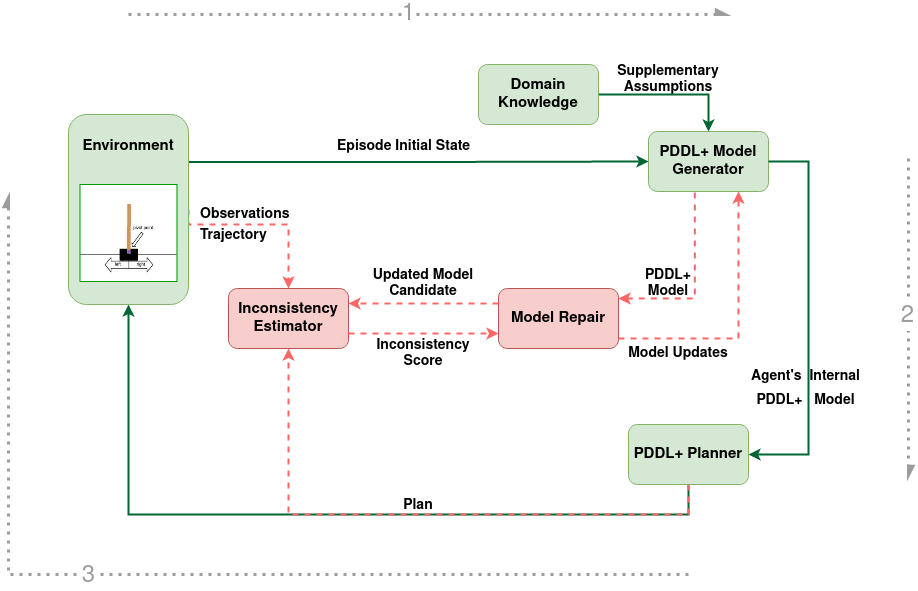
\includegraphics[width=\columnwidth]{./figures/repair_architecture_guide.png}
	\caption{Diagram of the agent's architecture for model repair. Note that, when using an accurate planning model $D$, only the green components are engaged. Once novelty is detected, however, the remaining repair-focused components (shown in pink) begin modifying the PDDL+ model.}
	\label{fig:repair_architecture}
\end{figure}

\begin{enumerate}
    \item \textbf{PDDL+ model generator.} At the beginning of an episode, the PDDL+ problem ($s_I$) is created by the PDDL+ model generator which takes as input a combination of the episode's initial state data from the environment and complementary assumptions about the environment. The problem is then paired with a PDDL+ domain file, hand-designed a priori, to compose the agent's internal PDDL+ model $D$. 
    \item \textbf{PDDL+ planner.} The agent attempts to solve the generated PDDL+ problem of the current episode, and stores the plan $\pi$.
    \item \textbf{Plan execution.} The agent sends the generated plan for execution inside the real-world environment ($D^*$).
    \item \textbf{Inconsistency estimator.} At the end of the episode, the agent computes the inconsistency score for the default model $D$ by comparing the expected state trajectory (obtained by simulating plan $\pi$) and the observed execution trace (trajectory $\tau$). 
    % Note that, for efficiency, this step can be conditional upon some criteria (e.g., if the last played episode ended in failure). 
    \item \textbf{Model repair.} If the inconsistency score exceeds a set threshold, the search-based model repair is engaged to adjust the agent's internal model $D$. The mechanism searches trough different candidate repairs to find one which sufficiently reduces inconsistency. The result is an updated model $D'$ which aligns with the real-world model $D^*$ such that the inconsistency score falls below the threshold once again.
    \item The agent moves on to the next episode and uses the updated internal model $D=D'$ to solve the subsequent tasks. The whole process repeats again from the start (1.).
\end{enumerate}

For clarity, note that the PDDL+ domain file describes general structure and system dynamics, and only needs to be defined once per environment. On the other hand, the PDDL+ problem is auto-generated per episode, combining the initial state data obtained from the environment and assumptions about the domain (i.e., values for variables that are required to accurately describe the environment and its dynamics, but which are not included in the data from the environment, e.g., gravity, velocities of moving entities).

% \roni{I recommend to shorten the above description of the PDDL+ model generator, just saying that it accepts the input from the environment and outputs a PDDL+ problem. Then explain all that is in the bullets there in a dedicated subsection or section.}

\section{Estimating Inconsistency}
%{\color{red}Planning with an incorrect or inaccurate domain model results in state changes in the environment that are different from with what was predicted by the planner during planning. Here we define an \emph{inconsistency} metric that captures the difference between two models numerically and is computed using execution traces. The inconsistency measure can be used to compare different repairs and select the one that is most accurate (as explained in the next section).} 


%Model repair needs to be able to compare different repairs and select the most accurate candidate. We define an inconsistency metric that estimates the difference between two models based on execution traces. In simple terms, the inconsistency metric measures the difference between the predictions of the planner and the observations gathered when executing the generated plan in the simulation environment.

% To account for the differences between simulation environments, the collected observations are translated into a common format that can be used for comparison against the expectations generated by the planner. 
% The observations are turned into a list of dictionaries where each element in the list represents a state in time of the environment, and contains a set of state variables (both propositional and numeric) paired with their values at the given time point. Note that, this is a lifted representation as the contents of the collected observations are limited to the information the simulation environment provides about its current state. The contents of the observations differ between environments but, in practice, they are usually what the human would see if they were interacting with it (e.g., types and spatial locations of the visible objects and entities). The received ground truth usually obscures information regarding the dynamics of the environment (e.g., velocities of objects, their masses, health-points). The obscured fluents are estimated or inferred in the planning model for completeness but these fluents are not used to compute the inconsistency between the planning expectations and simulation observations. In other words, inconsistency is only computed on the part of the set of state variables that can be directly mapped to corresponding true values in the true environment $D^*$.

Inconsistency metric $C \in \mathbb{R}_{\ge 0}$ is a measure of how accurately the planning model $D$ describes the actual environment and its dynamics $D^*$. It is computed using two aligned trajectories. One is obtained by simulating\footnote{Plan simulation can be done using dedicated plan simulators such as VAL~\cite{howey2004val}. In our work, we wrote our own Python-based general-purpose PDDL+ simulator used across various domains.} the generated plan $\pi$ and the PDDL+ model $D$, and the other trajectory $\tau$ is generated by the environment upon executing the plan $\pi$. Inconsistency is the sum of Euclidean distances between pairs of corresponding states in simulated and observed trajectories discounted proportionally by time. 

%We collect the expected states from simulating the generated plan $\pi$ (using model $D$) and align them against states in the observed trajectory $\tau$ (generated by the environment using real model $D^*$). 
% Note, that in cases where time is synchronized in the simulation and planning sides, aligning the two trajectories is trivial, but if common temporal information is not available, other alignment techniques need to be used.

%Inconsistency metric $C \in \mathbb{R}_{\ge 0}$ is a measure of how accurately the planning model $D$ of the environment $D^*$ describes the actual environment and its dynamics.
%Given a PDDL+ model $D$ and plan $\pi$, one can simulate\footnote{Plan simulation can be done using dedicated plan simulators such as VAL~\cite{howey2004val}. In our work, we wrote our own Python-based general-purpose PDDL+ simulator used across various domains.} the trajectory we \emph{expect} to observe when executing $\pi$.
%Our implementation of the Consistency Checking module computes the inconsistency score of an expected trajectory by measuring how different it is from the observed trajectory.
Formally, let $S(\tau)$ be the sequence of states in the observed trajectory and $S(\pi,D)$ be the expected sequence of states obtained by simulating the generated plan $\pi$ with respect to the agent's internal PDDL+ model $D$. Let $S(x)[i]$ denote the $i^{th}$ state in the state sequence $S(x)$. Inconsistency score of domain $D$ is computed as:
\begin{equation}
    C(\pi, D, \tau) = \sum_{i} \gamma^i\cdot ||S(\tau)[i] - S(\pi,D)[i]||
\end{equation}
where $0<\gamma<1$ is the discount factor. Errors can arise due to sensing noise, rounding errors, and other issues and can accumulate over time. Consequently, the Euclidean distance between corresponding states is likely to be higher later in the trajectories. The discount factor $\gamma$ prevents such errors from dominating the inconsistency estimation.  

%We define inconsistency as the sum of Euclidean distances between pairs of corresponding states, one from the expected state trajectory (i.e., executing plan $\pi$ in domain $D$) and one from the observed trace (i.e., from executing plan $\pi$ in real-world domain $D^*$). 

%To account for a possible accumulation of error over time due to noise and inherent planning model inaccuracies, the inconsistency scores are discounted proportionally with time. In other words, the inconsistency scores are more likely to be higher later in the state trajectory due to cumulative errors building up over time. We multiply the absolute inconsistency scores by a discount factor to prevent general model inaccuracies from dominating the inconsistency estimation. Discounting of later inconsistency scores also biases the mechanism to favor earlier inconsistencies with higher confidence. 


%Formally, let $S(\tau)$ be the sequence of states in the observed trajectory and $S(\pi,D)$ be the expected sequence of states obtained by simulating the generated plan $\pi$ with respect to the agent's internal PDDL+ model $D$. 
%Let $S(x)[i]$ denote the $i^{th}$ state in the state sequence $S(x)$. 
%The inconsistency score we considered is computed as follows:
%\begin{equation}
%    \sum_{i} \gamma^i\cdot ||S(\tau)[i] - S(\pi,D)[i]||
%\end{equation}
%where $0<\gamma<1$ is the discount factor. 

% In our implementation, we measured difference by computing the maximal Euclidean distance 
% between matching states along these trajectories (i.e., tracking differences between the \textit{expected} and \textit{observed} positions and velocities of the cart and pole over the course of an episode). 
% However, other ways to measure distances between trajectories can also be applied. 
% A novelty is detected when the discrepancy between the observed and expected sequence of states exceeds a predefined threshold. 

In a non-novel environment, the expected evolution of the system predicted by the planner should perfectly match the observed behavior in simulation, i.e., the two resulting trajectories should align by default with the inconsistency score $C=0$. In the real world, however, this is usually impossible to achieve due to rounding errors, perception inaccuracies, and similar common issues. To account for such noise, a domain-specific consistency threshold $T$ is set. A model $D$ is inconsistent with $D^*$ if $C(\pi, D, \tau) \ge T$ and consistent otherwise. Setting $T$ requires striking a fine balance between accurately estimating inconsistency and suppressing noise stemming from the execution environment.


%Thus, model $D$ is consistent with real model $D^*$ if its inconsistency score $C$ measured over plan $\pi$ is below the consistency threshold $C<T$. Conversely, model $D$ is inconsistent if its inconsistency score exceeds the threshold $C \ge T$ indicating that the environment was affected by novelty. Therefore, setting the consistency threshold requires a fine balance to accurately detect novelty while suppressing inconsistencies caused by the inherent noise from the environment. 
% A novelty is detected when the discrepancy between the observed and expected sequence of states exceeds the predefined threshold. 
A graphical representation of state trajectory-based inconsistency computation is shown in Figure~\ref{fig:inconsistency_trajectory} in which the expected state trajectory (purple nodes) is compared against the observed trajectory (green nodes). The gray dotted arrows denote the Euclidean distance between the observed state and the matching expected state generated by the planner using the agent's internal PDDL+ model $D$. The model $D$ is deemed inconsistent if the inconsistency threshold is exceeded. Note that while the inconsistency threshold is fixed, in the figure the threshold line rises over time. This is equivalent to the discount being applied to individual inconsistency scores. 
% This display choice avoids cluttering the graph, and helps in visualizing the influence of the inconsistency discount increasing with time.\roni{Last sentence is redundant and should be removed}





\begin{figure}
	\centering
	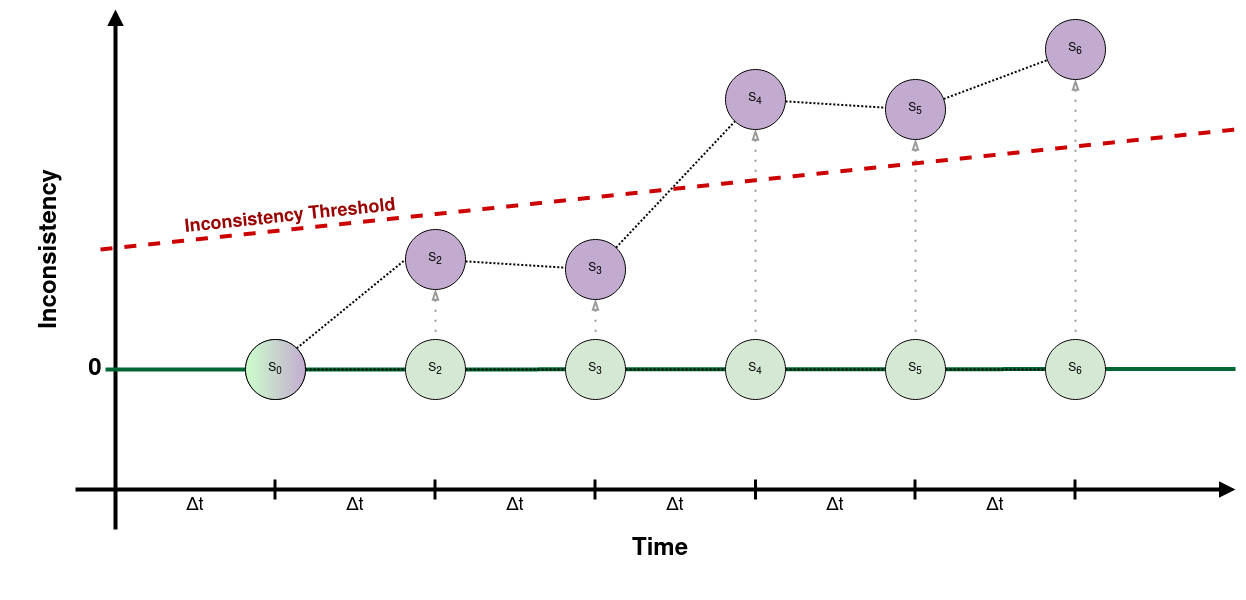
\includegraphics[width=\columnwidth]{./figures/trajectory_inconsistency2.png}
	\caption{Graphical representation of inconsistency of the expected state trajectory obtained from the generated plan by using the agent's internal model $D$ (purple nodes) with respect to the observations trajectory $\tau$ from the environment $D^*$ (green nodes).}
	\label{fig:inconsistency_trajectory}
\end{figure}

% This approach to detecting novelties is domain-independent, though, it relies on the accuracy of the planning model. 
% In our implementation, this was sufficient for our benchmark domains used in this paper. 
% However, for other domains the available PDDL+ model may not be accurate enough to exactly match the observed state trajectory. 
% %Note that it was accurate enough to allow the off-the-shelf PDDL+ planner to create plans that yielded state-of-the-art results in the non-novelty version of \sbirds. 


% To address this, one may augment the PDDL+-based Consistency Checking approach by creating a domain-specific consistency checking module that incorporates qualitative analysis of the observed and expected trajectories. Alternatively, one may employ representation learning and train a neural network over non-novelty episodes to do next state prediction. 



\section{Search-Based Model Repair}


% \subsection{Adapting to Novelty as Search in the Space of PDDL+ Models}
% The key to implementing a PDDL+-based \hydra agent is to define appropriate MMOs. 
% For a PDDL+-based \hydra agent, an MMO is a function that modifies some element of the PDDL+ model, e.g., change an action, event, or process, or even add a completely new event or process. 
% In our implementation, we limited the MMOs we consider to only modify the different constants used in the PDDL+ model, e.g., changing the constant corresponding to gravity by some fixed amount (either positive or negative). 

% The proposed search-based model repair algorithm works by searching for a \emph{domain repair}, which is a function that when applied to the agent's internal domain $D$, returns a domain $D'$ that is consistent with the observed trajectories. 
% To find such a domain repair, our algorithm accepts as input a set of basic \emph{Model Manipulation Operators} (MMOs), denoted $\{\varphi_i\}_i$. 
% Each MMO represents a possible change to the domain, e.g., increasing a domain fluent \roni{I think that maybe ``fluent'' is not the right word here and ``constant'' is better. What do you think?} by some fixed amount (denoted as $\Delta \in \mathbb{R}$). In general, we can define an MMO for any fluent $x \in X$ in the agent's internal model $D$ that is not directly mapped onto variables given by the environment (since they are the ground truth, $GT \subseteq X$, and are assumed to be accurate). 
% In practice, however, not all domain fluents are equal in their importance. 
% Domain knowledge can be exploited to analyze the level of impact each variable will have when its value is adjusted. Such analysis can be used to restrict the size of the set of \emph{repairable fluents} for improved efficiency of the overall algorithm. 
% More formally, the set of repairable fluents is defined as $RF \subseteq X \setminus GT$. 
% \roni{I think there was a bit of confusion between MMO, $\Delta$, and repairable fluents. I commented the original version above and propose the following. Your call.} 

The proposed search-based model repair algorithm works by searching for a \emph{domain repair} $\varPhi$, which is a sequence of model modifications that, when applied to the agent's internal domain $D$, returns a domain $D'$ that is consistent with the observed trajectories.
To find such a domain repair, our algorithm accepts as input a set of all possible basic \emph{Model Manipulation Operators} (MMOs), denoted $\{\varphi\} = \{\varphi_0, \varphi_1, ... , \varphi_n\}$. Each MMO $\varphi_i \in \{\varphi\}$ represents a possible change to the domain. Thus, a domain repair $\varPhi$ is a sequence of one or more basic MMO $\varphi_i \in \{\varphi\}$. An example of an MMO is to add a fixed amount $\Delta\in\mathbb{R}$ to one of the numeric domain fluents.
In general, one can define such an MMO for every domain fluent. In practice, however, not all domain fluents are equal in their importance. 
% Domain knowledge can be exploited to analyze the level of impact of adjusting the value of each fluent. Such analysis can be used to restrict the set of domain fluents for which we create MMOs of this type. 
The proposed search-based model repair algorithm works by searching for a \emph{domain repair} $\varPhi$, which is a sequence of model modifications that, when applied to the agent's internal domain $D$, returns a domain $D'$ that is consistent with the observed trajectories.
To find such a domain repair, our algorithm accepts as input a set of all possible basic \emph{Model Manipulation Operators} (MMOs), denoted $\{\varphi\} = \{\varphi_0, \varphi_1, ... , \varphi_n\}$. Each MMO $\varphi_i \in \{\varphi\}$ represents a possible change to the domain. Thus, a domain repair $\varPhi$ is a sequence of one or more basic MMO $\varphi_i \in \{\varphi\}$. An example of an MMO is to add a fixed amount $\Delta\in\mathbb{R}$ to one of the numeric domain fluents.
In general, one can define such an MMO for every domain fluent. In practice, however, not all domain fluents are equal in their importance. 


\begin{algorithm2e}
\SetKwInOut{Input}{Input}\SetKwInOut{Output}{Output}
% \SetKwComment{Comment}{$\triangleright$\ }{}
\Input{$\{\varphi\}$, a set of basic MMOs}
\Input{$D$, the original PDDL+ domain}
\Input{$\pi$, plan generated using $D$}
\Input{$\tau$, a trajectory}
\Input{$T$, consistency threshold}
\Output{$\varPhi_{best}$, a domain repair for $D$}
OPEN$\gets\{\emptyset\}$; 
$C_{best}\gets\infty$;
$\varphi_{best}\gets\emptyset$\\
\While{$C_{best}\geq T$}{
    $\varPhi\gets$ pop from OPEN\\
    \ForEach{$\varphi_i\in\{\varphi\}$}{
        $\varPhi'\gets \varPhi \cup \varphi_i$ {\scriptsize \tcc*{Compose a domain repair}} 
        DoRepair($\varPhi'$, $D$)\\
        $C_{\varPhi'}\gets$ InconsistencyEstimator($\pi$, $D$, $\tau$)\\
        \If{$C_\varPhi\leq C_{best}$}{
            $C_{best}\gets C_{\varPhi'}$\\
            $\varPhi_{best}\gets\varPhi'$
        }
        Insert $\varPhi'$ to OPEN with key $f(\varPhi', C_{\varPhi'})$ \nllabel{alg:line:f}\\
        UndoRepair($\varPhi'$, $D$)
    }
}
\Return $\varPhi_{best}$\\
\caption{PDDL+ model repair algorithm.}
\label{alg:repair}
\end{algorithm2e}


Algorithm~\ref{alg:repair} lists the pseudo-code for our search-based model repair algorithm. 
Initially, the open list ($OPEN$) includes a single node representing the empty repair, 
and the best repair seen so far $\varPhi_{best}$ is initialized to an empty sequence. 
This corresponds to not repairing the agent's internal domain at all. 
Then, in every iteration the best repair in OPEN is popped, and we compose new repairs by adding a single MMO to this repair, and add them to $OPEN$.  
For every such candidate repair $\varPhi'$ we compute a consistency score $C_{\varPhi'}$. 
This is done by modifying the agent's internal domain $D$ with repair $\varPhi'$, simulating the actions in plan $\pi$, and measuring the difference between the simulated outcome of these actions and the observed trajectory $\tau$. 
The consistency score $C_{\varPhi'}$ serves two purposes. First, we keep track of the best repair generated so far, and return it when the search halts. Second, we consider a repair's consistency score when choosing which repair to pop from $OPEN$ in each iteration. This is embodied in the function $f(\varPhi', C_{\varPhi'})$ in line~\ref{alg:line:f} in Algorithm~\ref{alg:repair}. 
In our implementation, $f$ is a linear combination of the consistency score the size of the repair, i.e., the number of MMOs it is composed of. The latter consideration biases the search towards simpler repairs. 

\begin{figure}
	\centering
	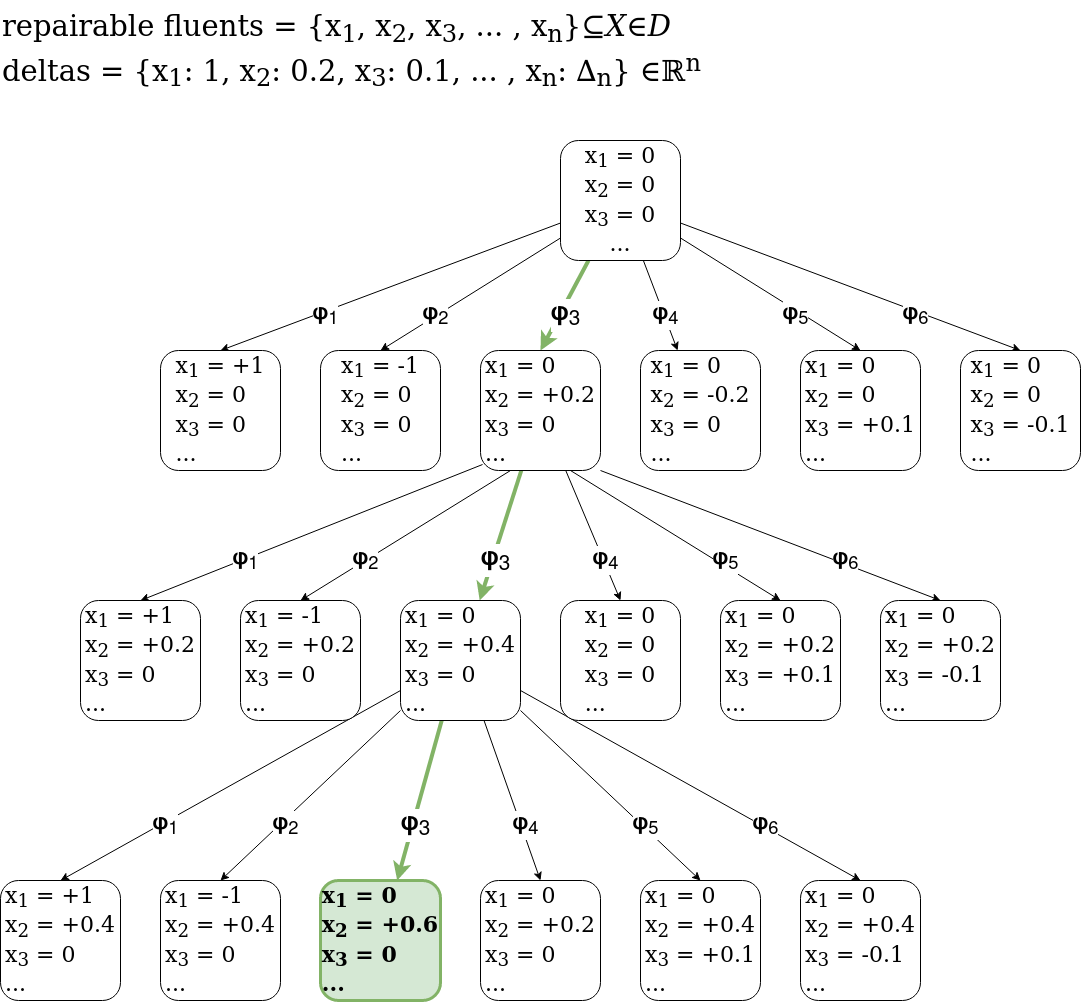
\includegraphics[width=\columnwidth]{./figures/MMO_search_tree3.png}
	\caption{An example MMO search graph showing how a repair (i.e., a sequence of MMOs) is selected. The green node depicts a goal state in the MMO repair search, the minimal change to the model that causes the inconsistency to fall below the set threshold.}
	\label{fig:mmo_search}
\end{figure}

Figure~\ref{fig:mmo_search} visualizes an example search tree of the MMO-based model repair algorithm where MMOs are treated as actions and the state is composed of changes to the default model (0 indicates no change to the given fluent). Inconsistency is estimated for each generated repair, and the search terminates once a repair is found such that the updated domain $D'$ is consistent with the true domain $D^*$. MMO repair is performed on a set of repairable fluents $\{x_1, x_2, ..., x_n\}$. Each MMO adjusts the value of a given fluent by a fixed amount $\Delta$ ($+\Delta$ or $-\Delta$), defined \emph{a priori} per fluent (denoted as delta in top left of Figure.~\ref{fig:mmo_search}). In this example scenario, the best repair $\varPhi_{best} = \{\varphie_3, \varphi_3, \varphi_3\}$ is a sequence of three MMOs (each adjusting $x_2$ by $+0.2$) such that repair $\varphi_{best}$ changes a single state variable $x_2 \in X$ by adding $0.6$ to its value.



\section{Experimental Evaluation}
\begin{figure*}
    \centering
    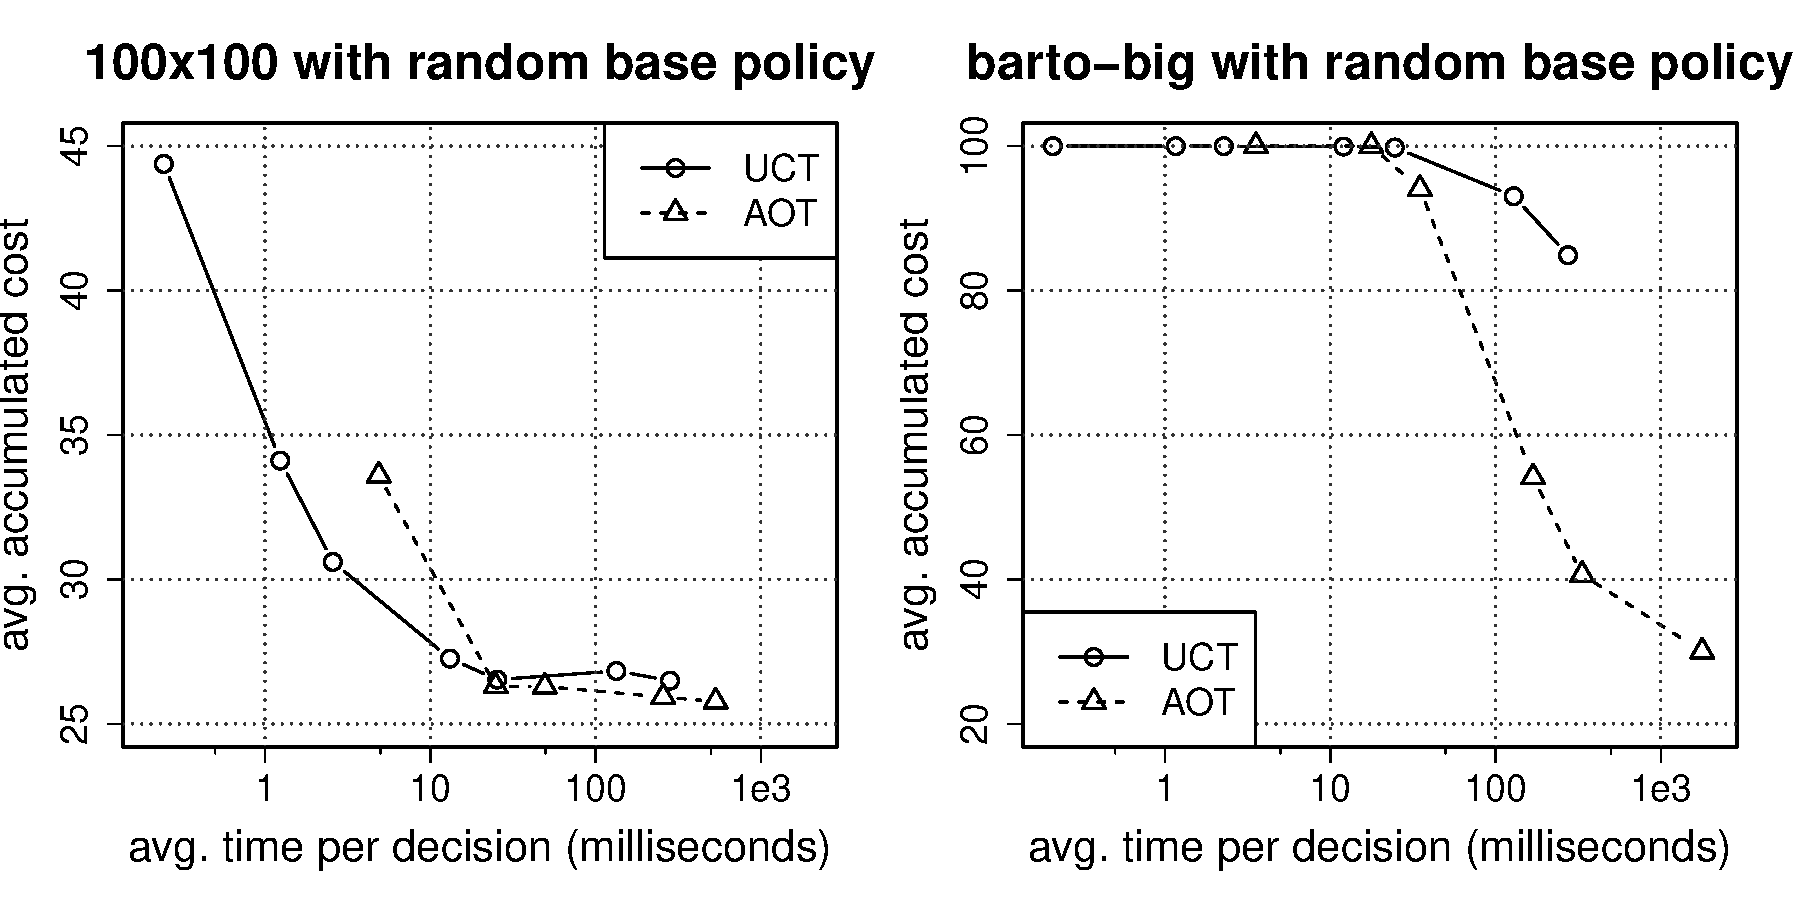
\includegraphics[width=1\textwidth]{./figures/experiments/combined.pdf}
    \caption{Graphs showing performance of DQN-static/adaptive and planning-static/repairing agents. Episodes in a trial are on the x-axis and reward earned is shown on the y-axis. The results are averaged over $5$ trials. Red line indicates the episode where environment parameters were changed.}
    \label{fig:combined_results}
\end{figure*}
In this section, we evaluate the efficacy of model repair in evolving environments and demonstrate its capability to improve an inaccurate model. We report results from two domains: CartPole and Angry Birds. CartPole is a well-known classical control and RL benchmark. We used the standard CartPole implementation provided by the OpenAI Gym\footnote{https://gym.openai.com}. Angry Birds is a popular mobile game that has featured as a domain in IJCAI competitions\footnote{http://aibirds.org/} since 2013. 

\subsection{Experiment 1: CartPole}
Our first set of experiments is designed to evaluate if the proposed model repair method can enable a planning agent to adapt to environment novelties. Recall that a novelty implies a sudden, unknown, and unexpected change in environment dynamics. In the CartPole domain, the agent's task is to balance the pole in the upright position for $n=200$ steps by pushing the cart either left or right. The domain's system dynamics are defined by several parameters: mass of the cart, mass of the pole, length of the pole, gravity, angle limit, cart limit, push force. The CartPole environment only provides information on the velocities and positions of the cart and the pole (4-tuple). The agent has two actions, left and right, that apply a constant force. Every step returns a $+1$ reward unless the pole diverges from vertical by $\pm 12^{\circ}$, at which point the episode ends in a loss. 

We structured our experiments as a set of $t=5$ trials consisting of $l=200$ episodes each. Each trial begins with episodes in nominal conditions. Novelty is introduced after $k=7$ canonical episodes where the environmental parameters are changed without informing the agent. Reward obtained by the agent in each episode is recorded.

\subsubsection{Agents}
We compared model-free reinforcement learning (RL) and model-based planning agents in our novelty experiments. Model-free RL agents were built with a standard deep Q-network implementation with experience replay memory \cite{mnih2013playing}. The Q-network is built with an input layer ($4 \times 16$), a hidden layer ($16 \times 16$), and an output layer ($16 \times 2$) and uses the Rectified Linear Unit (ReLU) activation function. The Q-network was trained to achieve perfect performance in the canonical setup prior to the experiments. The \emph{DQN-static} agent applies the policy learned in the canonical setup in the novelty setup. This baseline was implemented to ascertain that the introduced novelty indeed impacts performance of the agent and motivates adaptation. The \emph{DQN-adaptive} agent updated its network weights and learned a policy for the novelty setup.

The model-based planning agents were built with PDDL+. The expressiveness of PDDL+ enabled us to holistically encode CartPole's system dynamics as a planning domain (without using any external functions/solvers). Despite inherent complexity, efficient modeling allowed the use of off-the-shelf PDDL+ planners to solve the resulting problems. The planners were required to handle non-linear dynamics, large numbers of active happenings, and long temporal horizons. In our work on CartPole and other domains, we have successfully tested UPMurphi~\cite{della2009upmurphi} and ENHSP~\cite{scala2016interval}, but we ultimately opted for a novel discretization-based PDDL+ planner that allows greater flexibility and customization (though, it relies on the same principles for solving PDDL+ problems as the other two planners). The planner solves full CartPole PDDL+ problems in approx. $0.1$ seconds using GBFS algorithm with a domain specific heuristic prioritizing ``safe" states (pole upright, low velocities, close to the center). \emph{Planning-static} agent uses the same PDDL+ model for both the canonical and novelty setup. \emph{Planning-adaptive} agent monitors plan execution and automatically repairs the PDDL+ model inconsistency is detected. \emph{Repairable fluents} are all parameters defining CartPole dynamics: mass of the cart, mass of the pole, length of the pole, gravity, angle limit, cart limit, push force. 


\subsection{Results}
We report our observations on two novelties: length of the pole is updated to $1.1$, gravity to $12$; and length of the pole to $1.1$ and mass of the cart is decreased to $0.9$. These novelties were selected because they impact agent performance for all agents significantly. The performance of of all agents is summarized in Figure \ref{fig:combined_results}. The columns delineate the learning v/s planning methods and the rows, their static and adaptive versions. In each graph, $x$-axis captures the episodes in a trial and the $y$-axis shows the total reward collected by the agent per episode, represented as the proportion of its score with a perfect controller. The red line indicates the episode where the selected novelty (shown in the graph title) was introduced. The shaded area represents the $95\%$ confidence interval computed over $5$ trials. 

As shown in Figure \ref{fig:combined_results}, all agents demonstrate perfect performance at the beginning of the trial and then experience a significant drop in performance as soon as the novelty is introduced (episode $8$). This drop demonstrates that the changes in the environment dynamics impacts the performance of all agents. There is variability in how each agent responds to the changes in the environment. 

\subsubsection{Resilience of model-based agents} 
The novelty-induced performance drop is more significant in learning agents. For both types of novelties, the performance of the DQN agents drops below $30\%$ of its value in the canonical setup. In contrast, the performance of the planning agents drop to $\approx50\%$. This difference can be explained by the agents' design. The planning agents' PDDL+ model defines the system dynamics in a general manner. Thus, it can still be sufficiently accurate in some conditions. In contrast, the DQN agent's learned policy is not general and is only applicable for much reduced subset of cases after novelty.

% The performance drop observed when novelty is introduced is more for the learning agents than for the planning agents. For both types of novelties, the performance of the DQN agents drops to approximately $<30\%$ of its value in the canonical setup. In contrast, the performance of the planning agents drop to $\approx50\%$. This difference can be explained by the agents' design. The model-based planning agents comprise of several independent components (written as PDDL+ constructs here). While some components may not accurately capture the changed environment dynamics, others are still relevant for action selection. In contrast, the knowledge that drives behavior in model-free learning systems like the deep Q-network is distributed and may not be fully re-purposed to drive behavior in an environment with changing dynamics.

\subsubsection{Quick adaptation via model-space search} As expected, after novelty is introduced, the static versions of the DQN and planning agents continue performing poorly, while the adaptive agents improve their performance over time. However, the time taken to improve differs greatly between the DQN-adaptive and planning-adaptive agents. 
Learning in DQN-adaptive is slow, requiring multiple interactions with the environment. In our experiments, DQN-adaptive took $\approx75$ episodes to reach $90\%$ of optimal performance as shown in Appendix \ref{appendix:A}, Fig.~\ref{fig:rl-long}. In contrast, the planning-adaptive agent recovers very quickly in $<20$ episodes for both novelties (Fig.~\ref{fig:combined_results}). This observation supports our central thesis: model-space search enables quick adaptation in dynamic environments because it can localize changes in the explicit model. Repair-based adaptation is scalable and can handle very impactful novelty changes in system dynamics from the canonical setup (shown in Appendix \ref{appendix:A}, Fig.~\ref{fig:repairing-gravity-20}). 

\subsubsection{Explainable by design}
The model repair mechanism proposes concrete changes to the agent's explicit PDDL+ model. Thus, adaptation in the planning-adaptive agent is \emph{explainable}. A model designer can inspect the proposed repair to understand why and how the novelty affected the agent's behavior. In contrast, learning in model-free systems such as DQN-adaptive cannot be interpreted directly. 

The following text shows the distinct repairs that were found by the planning-repairing agent using the method proposed in this paper. Note that the reported values are changes from the nominal values used in the model. \\
\\
\begin{console}
\small
     \textbf{Repair 1:} {mass\_cart: 0, length\_pole: 0.3, mass\_pole: 0, force\_mag: 0, gravity: 0, angle\_limit: 0, x\_limit: 0} \\
    \textbf{Repair 2:} {mass\_cart: 0, length\_pole: 0, mass\_pole: 0, f
The model-based planning agents worce\_mag: 0, gravity: 1.0, angle\_limit: 0, x\_limit: 0}
    \\
    \textbf{Repair 3:} {mass\_cart: 0, length\_pole: -0.1, mass\_pole: -0.1, force\_mag: -1.0, gravity: 0, angle\_limit: 0, x\_limit: 0}
\end{console}
\smallskip
Despite these repairs being different from each other, the agent's performance converged to optimal with each one. One potential reason is that there are equivalence classes in the set of environmental parameters and their values. The agent uses only its observations over one episode in the environment to guide its search. It is likely that the observations by themselves do not provide sufficient information to determine the parameter values exactly and only differentiate between equivalence classes. 
% An analytical analysis of equivalence classes in CartPole parameters is out-of-scope for this paper. 

\subsection{Experiment 2}
Next we evaluate if the proposed method can alleviate inaccuracies in domain modeling by using observed data from execution. This test was done in Angry Birds. The objective in Angry Birds is to destroy pigs by launching birds at them from a sling-shot (shown in Figure \ref{fig:ab_level}). The launched birds obey the laws of motion and gravity. It is a difficult problem as it requires predicting outcomes of physics-based actions without having complete knowledge of the world, and then selecting an appropriate action out of infinitely many possible options. An Angry Birds level is \emph{passed} when all the pigs have been destroyed. 

\begin{figure}
    \centering
    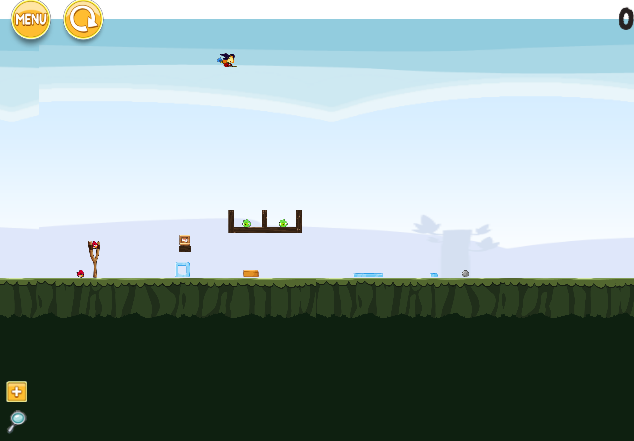
\includegraphics[width=0.9\columnwidth]{./figures/sb_level.png}
    \caption{Angry Birds Level used in our experiment}
    \label{fig:ab_level}
\end{figure}


Our tests were conducted in a specific subset of Angry Birds levels containing a small number of birds, blocks, and pigs (a sample is shown in Figure \ref{fig:ab_level}). We implemented a competent \emph{planning-static} agent using PDDL+. The PDDL+ model includes dynamics of launching a bird at maximum velocity at a certain angle, motion of birds and blocks, collisions between various objects, etc. The \emph{planning-adaptive} agent engages repair of the PDDL+ model when its observations become inconsistent with its expectations. We conducted $11$ trials of $25$ levels each. To simulate inaccuracies in modeling that invariably creep in during model design phase, we deliberately encoded incorrect values for certain parameters in the agents. Specifically, we reduced the maximum bird velocity by $4$ from its canonical value of $v_{bird}=186$. We measured how frequently each agent passes levels in a trial or the \emph{win rate}. 
% The minimum possible win rate is $0$ (when no level in a trial is passed) and the maximum is $25$ (when all levels are passed). 
We report the mean win rate for each agent and the $95\%$ confidence interval. 

The planning-static agent scored $0\% (0\%, 0\%)$ showing that the inaccuracy introduced in the model drastically degraded its performance. The planning-adaptive agent scored $52.36\% (28.72\%, 75.96\%)$ indicating that the proposed repair mechanism can alleviate inaccuracies in the agent's model and improve its performance significantly.

% The planning-static agent scored $0 (0, 0)$ showing that the inaccuracy introduced in the model drastically degraded its performance. The planning-adaptive agent scored $13.09 (7.18, 18.99)$ suggesting that the proposed framework can alleviate inaccuracies in the model and improve the agent's performance significantly. 

The results from CartPole and Angry Birds demonstrate that our proposed approach is applicable diverse scenarios. They highlight that not only the proposed approach can be used to develop robust planning agents that can handle sudden changes in the environment, it can also be used to improve accuracy of models of environment dynamics starting from rough approximations. 

\section{Conclusions and Future Work}
Realistic dynamical environments require building planning models without perfect information or full observability of the target environment. Additionally, in such scenarios, unexpected novelty can be introduced, significantly impacting the environment's features and dynamics in unknown ways. Such novelties can render any existing planning models obsolete, resulting in plan execution failures.


In this paper, we presented a domain-independent approach to model repair using heuristic search which enables autonomous agents to reason with novelties and mitigate their impact on the agent's performance. The approach works to correct inaccuracies in the agent's internal PDDL model based by measuring inconsistencies between its own planned expectations and observations from the execution environment. A state-based search algorithm guided by an inconsistency-based heuristic searches through different combinations of model modifications to find a viable repair which accounts for the novelty interference. We demonstrated our approach on complex PDDL+ domains, proving its applicability to realistic applications. Additionally, the presented approach can be used to design more accurate PDDL models by helping to find exact values of environmental parameters starting from rough approximations. 

To the best of our knowledge, this is the first attempt at model repair in state-based AI Planning, with previous works relating to plan execution failures choosing to focus largely on plan repair or replanning strategies. 

Future work will concentrate on automatically defining the set of repairable fluents and corresponding deltas, and improving the accuracy of the inconsistency metric. In the next stage, we will extend model repair to include modifications to the structure of the PDDL domain by adding, removing, and modifying preconditions, effects, and entire happenings.


% Use \bibliography{yourbibfile} instead or the References section will not appear in your paper
\bibliography{library}
% \pagebreak
% \appendix
% \section{Appendix A}
% \label{appendix:A}
% \begin{figure}[H]
%     \centering
%     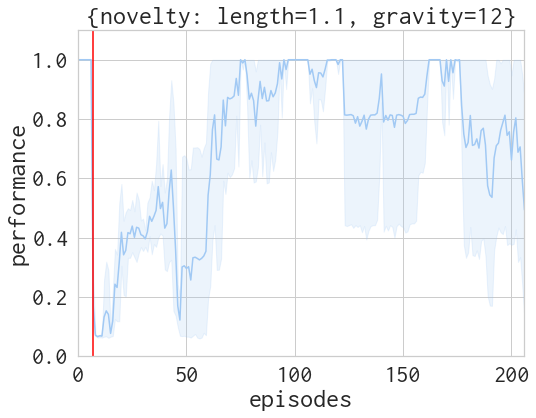
\includegraphics[width=1\columnwidth]{figures/experiments/rl_gravity_12_long.png}
%     \caption{Graph showing the number of episodes DQN-adaptive agent requires to learn a policy for optimal performance. The experimental setup is similar to what is described in the paper.}
%     \label{fig:rl-long}
% \end{figure}

% \begin{figure}[H]
%     \centering
%     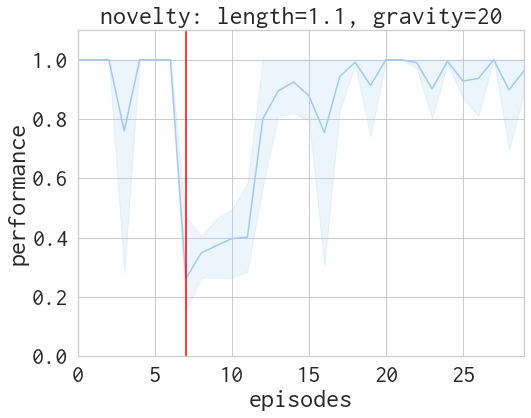
\includegraphics[width=1\columnwidth]{figures/experiments/repairing_gravity_20.png}
%     \caption{Graph demonstrating quick adaptation in the planning-repairing agent when the length of the pole was changed to $1.1$ and the gravity parameter was changed to more than twice its canonical value: $20$ in the novelty setting. The experimental setup is similar to what is described in the paper.}
%     \label{fig:repairing-gravity-20}
% \end{figure}

\end{document}


\end{document}